\documentclass{article}
\usepackage[utf8]{inputenc}
\usepackage[margin=1.0in]{geometry}
\geometry{letterpaper}
 
\usepackage{lscape}
\usepackage{dirtytalk}
\usepackage{mathtools}
\usepackage{titletoc}
\usepackage{minted}
\usemintedstyle{vs}
\setminted{fontsize=\small,baselinestretch=1}
\usepackage[natbibapa, sectionbib]{apacite}

\usepackage{url}
\usepackage[toc]{glossaries}
\makeglossaries
\usepackage{graphicx}
\graphicspath{ {./img/} }
\usepackage{comment}

\usepackage{listings}
\usepackage{color}
\usepackage[final]{pdfpages}
\definecolor{dkgreen}{rgb}{0,0.6,0}
\definecolor{gray}{rgb}{0.5,0.5,0.5}
%#EC7600
\definecolor{comment}{rgb}{.39,.45,.48}
\definecolor{number}{rgb}{1.0, 0.80, 0.13}
\definecolor{string}{rgb}{0.93,0.46,0.0}
\definecolor{keyword}{rgb}{0.58,0.78,0.39}
\definecolor{mauve}{rgb}{0.58,0,0.82}
\newenvironment{changemargin}{%
\begin{list}{}{%
    \setlength{\topmargin}{-1.0in}%
    \setlength{\leftmargin}{-0.5in}%
}%
\item[]}{\end{list}}

\lstset{frame=tb,
  language=C,
  aboveskip=3mm,
  belowskip=3mm,
  showstringspaces=false,
  columns=flexible,
  basicstyle={\small\ttfamily},
  numbers=none,
  numberstyle=\tiny\color{gray},
  %numberstyle=\tiny\color{number},
  keywordstyle=\color{blue},
  %keywordstyle=\color{keyword},
  %commentstyle=\color{comment},
  commentstyle=\color{dkgreen},
  stringstyle=\color{mauve},
  %stringstyle=\color{string},
  breaklines=true,
  breakatwhitespace=true,
  tabsize=3
}

\DeclarePairedDelimiter{\ceil}{\lceil}{\rceil}
\title{\gls{gpu} Acceleration of Audio Processing}
\author{Cindy Bui}
\date{December 19, 2018}

\setacronymstyle{long-short}  

\newacronym{api}{API}{Application Programming Interface}
\newacronym{cgma}{CGMA}{Compute to Global Memory Access}
\newacronym{cpu}{CPU}{Central Processing Unit} 
\newacronym{dft}{DFT}{Discrete Fourier Transform}
\newacronym{dsp}{DSP}{Digital Signal Processing}
\newacronym{fft}{FFT}{Fast Fourier Transform}
\newacronym{eq}{EQ}{Equalization}
\newacronym{fir}{FIR} {Finite Impulse Response}
\newacronym{flops}{FLOPS}{Floating Point Operations Per Second}
\newacronym{gflops}{GFLOPS}{Giga Floating Point Operations Per Second}
\newacronym{gpu}{GPU}{Graphics Processing Unit}  
\newacronym{hrtf}{HRTF}{Head Related Transfer Function}
\newacronym{hpc}{HPC}{High Performance Computing}
\newacronym{lsi}{LSI}{Linear, Shift-Invariant}
\newacronym{sm}{SM}{streaming multiprocessor}
\newacronym{sp}{SP}{streaming processor}
\newacronym{pcie}{PCIe}{Peripheral Component Interconnect Express}







\newglossaryentry{cuda}{name=CUDA, description=An API and platform developed by NVIDIA for GPU programming. Stands for Compute Unified Device Architecture}
\newglossaryentry{execution configuration}{name=execution configuration, description=dimensions of the grid and block that are necessary before a kernel call}
\begin{document}


%titlepage
\thispagestyle{empty}
\begin{center}
\begin{minipage}{1.0\linewidth}
    \centering
%University logo
    
\includegraphics[width=0.50\linewidth]{nyu_long_color.png}
    %\rule{0.4\linewidth}{0.15\linewidth}
    \par
    \vspace{2.5cm}
%Thesis title
    {\uppercase{\Large GPU Acceleration of Massive Convolution \par}}
    \vspace{2.5cm}
%Author's name
    {\Large Cindy Bui\par}
    \vspace{2.5cm}
%Degree
    {\Large NYU Steinhardt Music Technology Undergraduate Capstone\par}
    \vspace{2.5cm}
%Credits
    {\Large Advice and Guidance: Dr. Brian McFee and Dr. Mohamed Zahran\par}
    \vspace{2.5cm}
%Date
    {\Large December 14, 2018}
\end{minipage}
\end{center}
\clearpage
\tableofcontents

\newpage


\section{Introduction}

\indent \par \gls{dsp} is a field of applied mathematics and physics on a collection of numbers known as samples. The entire collection of these samples emulate the shape of the voltage sent to a speaker to play audio or voltage received from a microphone. Once these samples are stored digitally, they can be modified in some shape or form. Then, these samples can be sent through a piece of hardware to be sent to a speaker to play music.

For example, multiplying every sample in this collection by 0.5 before sending the signal to a speaker will cut the amplitude in half, effectively making the signal sound 6 dB quieter.

Basic \gls{dsp}, such as the above example of gain reduction, is in every device that can play audio and record it, like phones and laptops. More complex \gls{dsp} techniques are in devices like mixing consoles and software such as Digital Audio Workstations.

Mixing consoles typically have dedicated hardware known as digital signal processors. These chips are especially built for \gls{dsp}, and they're designed to do arithmetic on samples extremely quickly. Audio sample rates are typically 44.1kHz, 48kHz, 96kHz, and 192kHz, which are the number of samples per second. The more samples there are per second, the higher the frequency resolution of the audio is. At the same time, that's more computations that processors have to compute per second. At the time of writing, the industry standard sample rate is in the process of moving from 48kHz to 96kHz. The drawback of moving to 96kHz is the doubling in computation time, which this paper will offer suggestions to enhance. Digital signal processors, because they are specialized for \gls{dsp}, are incredibly fast and can handle 96kHz or 192kHz with no problem, but they are only found in specific hardware.

On a computer, the \gls{cpu} typically does all of the processing. While this chip is powerful enough to perform \gls{dsp} on large amounts of audio, the problem is that the \gls{cpu} also has to multitask and run other programs at the same time. The operating system itself of a computer is a massive, resource-intensive piece of software. Any interactive, click-and-point interface also requires resources. In addition, the way that the \gls{cpu} is designed, it is supposed to have average efficiency for all possible tasks thrown at it, which doesn't make it the most effective hardware for \gls{dsp}.

This research project aims to offload the work of \gls{dsp} onto a different chip, the \gls{gpu}, and to compare the performance results to that of a \gls{cpu}. The two chips are designed to do arithmetic and computations, but the primary difference is that a \gls{gpu} is designed to do computations in parallel where a \gls{cpu} is designed to do computations sequentially. Meaning, a \gls{gpu} is designed to do thousands of tasks at the same time at an overall slower rate, where a \gls{cpu} is designed to do tasks one after the other incredibly quickly.

I am testing one of the most computationally expensive \gls{dsp} operations - massive convolution - on a \gls{cpu} and a \gls{gpu}. The goal is to benchmark them and see at what point it's better to use which chip.


\section{Background}
\subsection{Digital Signal Processing Background}
\indent \par Massive convolution is a type of convolution with very large inputs - in the realm of millions of samples or more.

Convolution itself is a mathematical operation that causes a signal's shape to be modified by another, typically smaller signal. For audio, it causes the frequency content of two signals to blend together. I'm going to refer to the signal to be convolved as the input signal and the smaller, shape-modifying signal as a filter.

In \gls{dsp}, convolution is the operation by which \gls{lsi} systems are implemented. A system is a general term for an operation on an input signal that results in a modified output signal. \gls{lsi} systems are combinations of delay and amplitude modulation. The audio filters implemented in this manner are called \gls{fir} filters. The most common \gls{fir} filters are \gls{eq} filters (such as low-pass, band-pass, and high-pass filters), binaural spatialization with \glspl{hrtf}, and adding reverberation to a signal. For EQ filters, the size of the filter increases with the quality of the filter. It can range from 10 samples to 680476 samples \citep{lopo_2011}. \gls{hrtf} filters vary between 128 to 512 samples \citep{andreopoulou2011towards}. 

For reverberation (reverb), the filter is typically how long it takes for an impulse or a sudden burst of sound to dissipate in a room. This used to be recorded by popping a balloon or shooting a starter pistol in a room. This is typically around 2 seconds long. At a sample rate of 96kHz, that would mean 192,000 samples. Having a 5 second reverb filter - which intuitively makes sense for a very reverberant room - would create a filter of 480,000 samples. Some impulses could even be 10-20 seconds long such as a gymnasium, so 960,000 - 19,200,000 samples long.

A 480,000 sample filter intuitively makes sense, however 460,800,000,000 computations are required to perform convolution with 480,000 samples on an input that is also 480,000 samples. This is because of the formula for full convolution:
\begin{center}
$$(x * h)[n] = y[n] = \sum_{k=0}^{K-1} x[n-k] \cdot h[k]$$
where $x =$ input signal, $h =$ filter

$\cdot$ is the arithmetic multiplication operator (normal multiplication)

$N =$ length of $x$, $K =$ length of $h$

$0 \leq n \le N + K - 1 <==> n = [0, N + K)$

all out-of-bounds values of $x$ are assumed to be 0\footnote{Through the entirety of this paper, I will represent the input as $x$, the filter as $h$, the length of $x$ as $N$, and the length of $h$ as $K$. $N$ will be used in other contexts as the number of elements, but these variables and future variables will refer to the same definition.}

\end{center}
\noindent $(x * h)$ means the convolution of $x$ and $h$, where $*$ is the convolution operator. Ignoring the corner-cases at the beginning and the end, this formula is saying that a single point of the output is the sum of each point of the filter multiplied by a point of the input. Each output value requires at most $K$ multiplies and $K - 1$ additions. The length of the output is $N + K - 1$. The number of calculations is therefore proportional to $(N + K - 1) \cdot (2K - 1) \propto 2K(N + K)$. Including the corner cases where there are 1 to $K - 1$ terms added together, the true number of multiplication and addition operations would be 

$$N \cdot K \cdot 2 = 460,800,000,000$$ 

The number of computations is proportional to the size of the input multiplied by the size of the filter, and the worse case scenario is if the filter and input are of the same length. In general, this means that the convolution operation, or more conceptually - the convolution algorithm -, is of the order $N^2$, notated as $O(N^2)$. 

By computer science standards, an algorithm with $O(N^2)$ is very slow. So, actual implementations of convolution utilize the Convolution Theorem which implement the Fourier transform (represented here by $F()$)

$$F(x * h)  = F(x) \cdot F(h)$$
$$(x * h) = F^{-1}(F(x) \cdot F(h))$$
This says that taking the Fourier transform of the input and filter, point-wise multiplying them together, and taking the inverse Fourier transform of the product is equivalent to taking the convolution of $x$ and $h$.

This is preferred because an implementation of the Fourier transform known as the \gls{fft}, or more specifically the widely used Cooley-Tukey FFT algorithm, has a computational complexity of $O(N\log_2{N})$ for input sizes that are a power of 2. 

Taking the \gls{fft} of two signals and multiplying them would result in a computational complexity of:

$$N\log_2{N} + N\log_2{N} + N$$
$$2N\log_2{N} + N $$
$$N\log_2{N}$$
For computational complexity, the coefficients are ignored and only the largest term in a polynomial is used, because they don't create much of an impact as $N$ grows infinitely large.

$O(N\log_2{N})$ has a significantly smaller growth rate than $O(N^2)$. For example, if $N = 480,000$, 
$$\ceil{480000\log_2{480000}} = 905,889$$
$$480000^2 = 230,400,000,000$$

This means that a frequency-domain convolution would take approximately 905 thousand computations, while a time-domain convolution would take 230 billion computations. As N grows, $N^2$ will become significantly larger than $N\log_2{N}$. However, performing the FFT is an overhead. For small filters and small inputs, time domain convolution will be faster. 

\vspace{5mm}

Unfortunately, all of the past examples have been 5 seconds worth of audio at 96kHz, or 10 seconds of audio at 48kHz. Actual audio inputs can be anywhere from 1 second to several days long. To put it in perspective, the movie \textit{Interstellar} is 2 hours and 49 minutes long. The entirety of \textit{Interstellar}, assuming it is in stereo and pretending that films use a sample rate of 96kHz, is 1,946,880,000 samples. Even thinking about $N\log_2{N}$ or $N^2$ of that number is frightening. This is why we use computers to do the math for us!

\subsection{Computer Science/Computer Engineering Background}
When writing programs that deals with audio, typically the samples are read as 32 bit floating-point numbers. This is due to programmer convenience - the math is easier, and the programmer doesn't have to worry about integer underflow or overflow.

There's a specification for processing units called \gls{flops} This number is generally in the range of billions, so they're further specified in whitepapers as \gls{gflops}. As an example let's take a 5th Generation Intel® (Codename Broadwell, primary architecture type codename Haswell) Core™ I5-5575R  processor, which was released in 2014 \citep{export_compliance}. The R means that it is a desktop CPU based off a mobile chip, and it contains high performance graphics \citep{intel}. Its peak theoretical number of \gls{gflops} is 179.2. This means that it can do theoretically do 179,200,000,000 floating point operations per second. It could convolve our 5 second audio with our 5 second reverb in about 0.005 milliseconds if using the frequency-domain convolution algorithm. It would take at least 2.5 seconds to do the same in the time domain. 

To give a massively larger estimate, let's plug in the number of samples in \textit{Interstellar} to the computational complexities of time domain and frequency domain convolution as an estimate of the number of computations, and then divide that by the number of GFLOPS on this CPU. I said before that \textit{Interstellar} has approximately 1,946,880,000 samples if it were recorded at 96kHz. I'm going to use $3N\log_2N + N$ in the frequency domain approximation of number of computations (two forward Fourier transforms, one pointwise multiplication, and one inverse Fourier transform). Here, $s$ means seconds and $c$ means computations.

$$ \frac{(1.94688 \cdot 10^9)^2 c}{179.2 \cdot 10^9  c/s} = 21,151,460.6s$$

\noindent 21,151,460.6 seconds = 352,524.343 minutes = 5,875.40572 hours = 244.808572 days $\approx$ 8 months and 5 days.

$$\frac{(3 \cdot 1.94688 \cdot 10^9)\log_2(1.94688 \cdot 10^9) + 1.94688 \cdot 10^9 c}{179.2 \cdot 10^9 c/s} = 1.01663152s$$

This is why we do convolution in the frequency domain!


The problem is that processors rarely ever reach peak performance for a single process or operation. The \gls{cpu} has to run an operating system at the same time, which is an extremely resource intensive software. In addition to that, there will be hardware latency in reading data to the \gls{cpu} and writing data. Since the \gls{cpu} operates sequentially, the \gls{cpu} can't do any computations while it's waiting to receive data or if there is a system call to the operating system. This causes massive slowdown - even if the processor is multi-core, meaning it has multiple \gls{cpu}'s inside of a single chip.\footnote{Programming for multi-core \gls{cpu}'s is another field that can be explored, but this paper will not deal with multi-core processing units} 

A \gls{gpu}, on the other hand, is designed to maximize \gls{gflops} by processing these computations in parallel. For example, take the Nvidia Tesla M40 graphics card (Generation codename Maxwell) which was also released in 2014. The Tesla series are the high end \glspl{gpu} meant for data centers and high performance computing. It has a theoretical peak of 6,840 \gls{gflops}, single-precision \citep{teslagp100}. Blindly inserting them into the previous equations:

$$\frac{(1.94688 \cdot 10^9)^2 c}{6.84 \cdot 10^12  c/s} = 554,143.528 s$$
554,143.528 seconds = 9,235.72547 minutes = 153.928758 hours = 6.41369825 days
$$\frac{(3 \cdot 1.94688 \cdot 10^9)\log_2(6.84 \cdot 10^12) + 1.94688 \cdot 10^9 c}{6.84 \cdot 10^12  c/s} = 0.0366922554 s$$

That's a \textit{significant} performance boost. However, peak \gls{gflops} comes with the caveat that it's almost impossible to reach. Getting anywhere close to the peak theoretical \gls{gflops} on a \gls{gpu} in performance requires specific programming techniques and computational thinking. 

The actual amount of time that these computations will take for either chip requires experimentation - trial and error. This paper is a culmination of a benchmarking test of both time domain and frequency domain convolution on a \gls{cpu} and \glspl{gpu}. The \gls{cpu} program is purely sequential, ignoring multi-core programming. Both programs are written in C with some C++, and the \gls{gpu} accelerated code uses NVIDIA's \gls{cuda} platform/\gls{api}.

\section{Project Description}
\subsection{Overall Algorithm}
I am reading the audio samples as 32 bit floating point numbers using the libsndfile library \citep{lopo_2013}. When writing audio files interpreted as floats, audio falls between -1.0 and 1.0. Due to the nature of discrete convolution, the output values will be significantly greater than the input and most likely exceed a peak of 1 because of the summation. It is required to scale the output so that the output audio doesn't clip, and this process is called normalization.

I chose peak normalization. The formula for peak normalization is to find the maximum value of the absolute value of the input signal and store it. After doing convolution, find the peak of the output. Then, multiply the entire output by the input peak divided by the output peak. 

\vspace{5mm}
\textbf{Generic FIR Convolution Algorithm}
\begin{enumerate}
   \item Read input wave file
   \item Read filter wave file
   \item Find peak of input
   \item Convolve the two signals
   \item Find peak of output
   \item Scale output according to the input
   \item (Optional) Write output to a file
\end{enumerate}



\subsection{Sequential Algorithm}
For sequential algorithms, the generic algorithm is expanded to look something like this:

\begin{minted}{cpp}
Generic Sequential Convolution Algorithm

read input.wav into x
read filter.wav into h
/*Find peak of input*/
peakIn = 0
for i in x:
    if | i | > peakIn:
        peakIn = i
        
/*Convolve*/
y = convolve(x,h)

/*Find peak of output*/
peakOut = 0
for i in y:
    if | i | > peakOut:
        peakOut = i
/*Scale all points in output*/
for n in y:
    n = n * peakIn / peakOut

/*(Optional) Write to output file*/
write y to output.wav
\end{minted}
\subsubsection{Time Domain Convolution}
\indent \par As explained in the background section, the equation for full convolution is:
$$y[n] = \sum_{k=0}^{K-1} x[n-k] \cdot h[k]$$

A direct transliteration of the summation, where $Y = N + K -1$ or the length of the output, would look like this:

\begin{minted}{cpp}
Direct Transliteration of Convolution Equation

for n [0, Y):
    y[n] = 0
    for k [0, K):
        if (n - k < N):
            y[n] += x[n - k] * h[k]
\end{minted}
The problem is that this has a high probability of cache misses. Cache is temporary storage inbetween memory and the \gls{cpu}. When a program asks for a value in an array or somewhere in memory, an entire block of memory (typically 64 bytes or 8 floating point numbers) is stored in the cache. This takes some extra time, but it becomes useful if the program utilizes the rest of the numbers in the block. The retrieval of the data from memory to cache takes longer than retrieval of data from cache to \gls{cpu}. Therefore, programs that access memory sequentially are more likely to be retrieving from cache with fewer trips to the main memory and are therefore faster. The previous code snippet had \verb|x[n-k]| where \verb|n| and \verb|k| increase, \verb|k| faster than \verb|n|. Because of this, \verb|x| is being accessed in reverse then jumping forward in time.


\begin{minted}{cpp}
Optimized Convolution Algorithm

/*Set all values in y to zero first*/
for n in y:
    n = 0
    
for k [0, K):
    for n [0, N):
        y[k + n] += x[n] * h[k]
\end{minted}
Where K = length of h and N is the length of x.

\noindent This was lightly tested for K = 480,000 and N = 2,304,000. All trials were done on different \gls{cpu}s, but each trial was done on the same \gls{cpu}. 

\begin{center}
Speed Benchmarks for Cache-Unfriendly vs Cache-Friendly
\begin{tabular}{ c c c c c }
 Trial Number & Cache Unfriendly & Cache Friendly & Speedup amount & Percent speedup (floor)\\ 
 1 & 4,878.2635 s & 3,292.94750 s & 1,585.61600 s & 32 \\  
 2 & 4,987.8665 s & 3,801.66950 s & 1,186.19700 s & 23 \\
 3 & 5,214.8175 s & 3,707.61700 s & 1,507.20050 s & 28 \\
 4 & 4,713.9980 s & 3,228.36475 s & 1,485.63325 s & 31 \\
 5 & 4,887.9455 s & 3,417.36225 s & 1,470.58325 s & 30
\end{tabular}
\end{center}

In audio terms, this input is tiny. At 96 kHz, it's only 24 seconds long. Longer inputs will have more drastic differences and larger percentages.

Taking the cache into account, my full time domain convolution algorithm looks like this:

\begin{minted}{cpp}
Time Domain Convolution Algorithm

read input.wav into x
read filter.wav into h
/*Find peak of input*/
peakIn = 0
for i in x:
    if | i | > peakIn:
        peakIn = i
        
/*Convolve*/
for n in y:
    n = 0
for k [0, K):
    for n [0, N):
        y[k + n] += x[n] * h[k]
        
/*Find peak of output*/
peakOut = 0
for i in y:
    if | i | > peakOut:
        peakOut = i
/*Scale all points in output*/
for n in y:
    n = n * peakIn / peakOut

/*(Optional) Write to output file*/
write y to output.wav
\end{minted}

\subsubsection{Frequency Domain Convolution}

Also stated in the background section, the formula for frequency domain convolution is:

$$y = F^{-1}(F(x) \cdot F(h))$$
\paragraph{Padding Considerations} \hspace{0pt} \\
\indent While the Fourier transform is not covered in this paper, there are several important aspects of the Fourier transform and the convolution theorem that affect the padding of the signal.

A crucial aspect of the \gls{dft} is that each index of the transformed, discrete signal corresponds to a certain analysis frequency, and the value of that index is the energy of that frequency. The analysis frequency at each index is determined by the number of samples of the pre-transformed/transformed signal and the sample rate of the audio. The implication of this is that the filter's frequency bins must align with the input's frequency bins in order for the pointwise multiplication to make sense. So the filter must be padded with 0's so that it is of length N before taking the \gls{dft} of the signal. 

As stated earlier, the FFT is a specific implementation of the \gls{dft} that reduces the number of necessary computations. This operates by a divide and conquer algorithm that will operate faster the lower the least prime factor of the input is. Meaning, the FFT is the fastest when the signal is a power of 2. To make the FFT perform faster, the two signals must be padded with zeroes to the next largest factor of 2. The padded length = $2^{\ceil{\log_2N}}$.

Lastly, the convolution theoreum states that pointwise multiplication in the frequency domain is convolution in the time domain but more specifically \textit{circular} convolution. Circular convolution is different from full convolution in how it changes the assumption about out of bounds values. The assumption for full convolution was that all out of bounds values of x are 0. Circular convolution makes the assumption that negative indices of x will refer to the end of x. $x[-K + 1:-1] = x[N - K: N - 1]$ Because data at the end of a signal doesn't usually relate to the beginning of a signal, we pad the input with at least K - 1 zeross to prevent the circularity and force those out of bounds values to become 0. 

\vspace{5mm}
After all of these considerations, the size of the padded FFT input($P$) should be $P = 2^{\ceil{\log_2(Y)}}$, where $Y = N + K - 1$.

\paragraph{FFTW3} \hspace{0pt} \\
\indent FFTW3 is the name of the Fourier transform library that I used. It provides memory allocation wrappers for complex inputs and real inputs to ensure that they are optimized for speed. Then, in order to execute a Fourier Transform, a plan needs to be created with the parameters for the transform. There are also specific \glspl{api} meant for the transform of one dimensional, real valued inputs. The library typically uses double precision floating point values. I'm choosing to use single precision floating point variant by putting "f" on the end of every \gls{api}. These are the \glspl{api} \citep{fftw3}.

\begin{minted}[breaklines, breakanywhere]{cpp}
Allocating memory
float * fftwf_alloc_real(size_t n);
fftwf_complex * fftwf_alloc_complex(size_t n);

Basic interface
fftwf_plan fftwf_plan_dft_r2c_1d(int n, float *in, fftwf_complex *out, unsigned flags);
fftwf_plan fftwf_plan_dft_c2r_1d(int n, fftwf_complex *in, float *out, unsigned flags);

Advanced interface
fftwf_plan fftwf_plan_many_dft_r2c(int rank, const int *n, int howmany, float *in, const int *inembed, int istride, int idist, fftwf_complex *out, const int *onembed, int ostride, int odist, unsigned flags);
fftwf_plan fftwf_plan_many_dft_c2r(int rank, const int *n, int howmany, fftwf_complex *in, const int *inembed, int istride, int idist, float *out, const int *onembed, int ostride, int odist, unsigned flags);

Basic Execution
void fftwf_execute(const fftw_plan plan);

Used to apply pre-existing plans to different arrays 
void fftwf_execute_dft_r2c(const fftwf_plan p, float *in, fftwf_complex * out);
void fftwf_execute_dft_c2r(const fftwf_plan p, fftwf_complex *in, float * out);

Cleanup
void fftwf_destroy_plan(fftw_plan plan);
void fftwf_free(void *p);
\end{minted}
Using the r2c and c2r is more efficient both in terms of number of computations and in memory. By using the r2c, this transform will only compute the first $\lfloor\frac{P}{2}\rfloor + 1$ terms of the transform. This utilizes the property of aliasing in audio. Aliasing is when one signal looks like a slower one because the sample rate is too low to properly represent it. Aliasing occurs when the frequency exceeds $\frac{1}{2}$ of the sample rate. The r2c doesn't even bother to compute the transform values past $\lfloor\frac{P}{2}\rfloor + 1$, cutting the amount of necessary computations in half. In addition, the output only contains  $\lfloor\frac{P}{2}\rfloor + 1$ numbers, which cuts the amount of memory for the output in half. c2r is the complimentary transform expecting $\lfloor\frac{P}{2}\rfloor + 1$ values and will return an output of $P$ values. 


\begin{changemargin}
\def\excerpt{\thispagestyle{empty} \paragraph{Frequency Domain Convolution Algorithm} \hspace{0pt} \\}
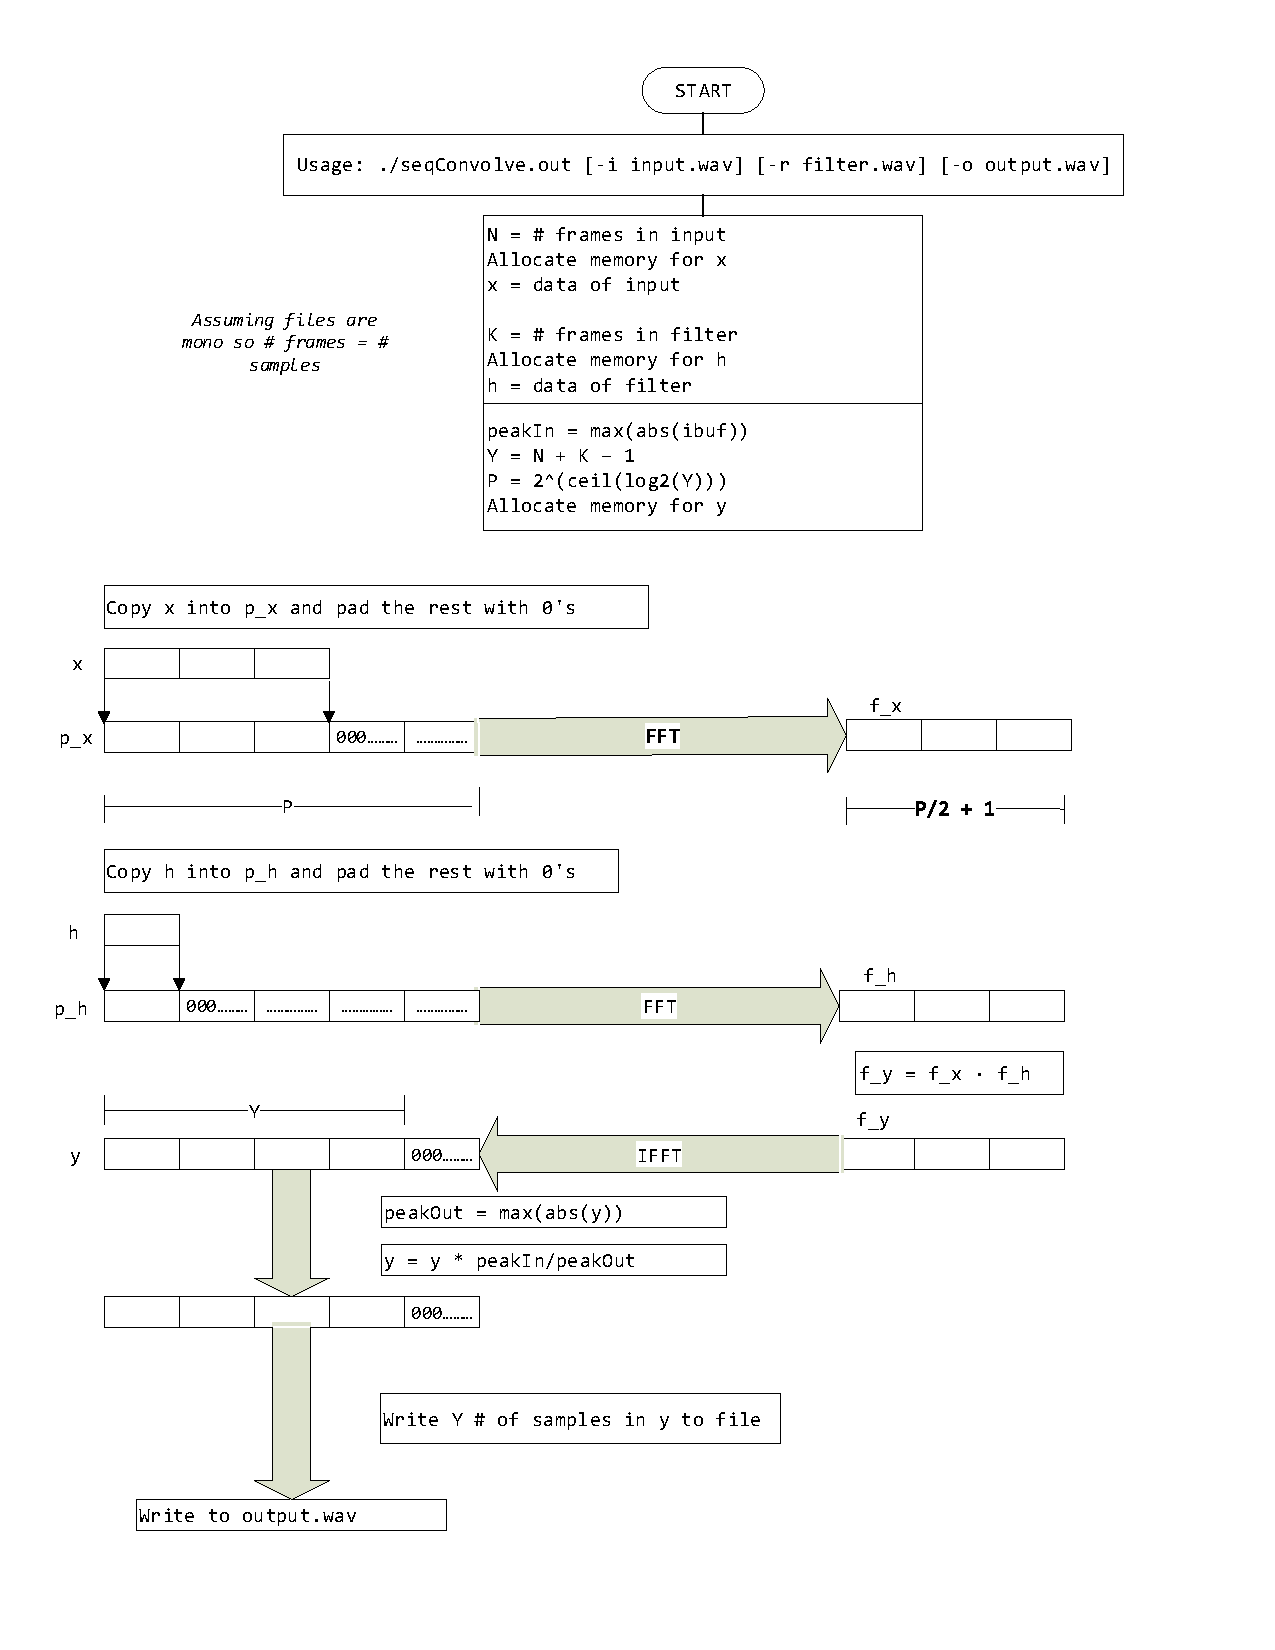
\includepdf[pages=1,pagecommand={\excerpt}]{Algorithms.pdf}
\end{changemargin}

\begin{minted}{cpp}
Frequency Domain Convolution Algorithm

read input.wav into x
read filter.wav into h
N = length of x
K = length of h

/*Find peak of input*/
peakIn = 0
for i in x:
    if | i | > peakIn:
        peakIn = i

/*Find length of output and padded length*/
Y = N + K - 1
P = pow(2, ceil(log2(Y)))

/*Copy x and h into p_x and p_h*/
p_x[0 : N - 1] = x
p_h[0 : K - 1] = h

/*Pad p_x and p_h with zeros*/
p_h[K : P - 1] = 0
p_x[N : P - 1] = 0

/*Take the Fourier transform*/
f_x = fft(x)
f_h = fft(h)

/*Convolution*/
f_y = f_x * f_h

/*Take the inverse Fourier transform*/
y = ifft(f_y)
        
/*Find peak of output*/
peakOut = 0
for i in y:
    if | i | > peakOut:
        peakOut = i
        
/*Scale all points in output*/
for n in y:
    n = n * peakIn / peakOut

/*(Optional) Write to output file*/
write y[0 : Y - 1] to output.wav
\end{minted}

\paragraph{Complex Multiplication} \hspace{0pt} \\
\indent An important point to note is that pointwise multiplication of the transformed signals is complex multiplication. C recognizes the complex number as a structure of two floats, so there needs to be a separate multiply function. 

$$(a_1 + b_1j) \cdot (a_2 + b_2j) = $$
$$a_1a_2 + a_1b_2j + a_2b_1j - b_1b_2 =$$
$$ a_1a_2 - b_1b_2 + a_1b_2j + a_2b_1j$$

The FFTW library incorporates a complex structure called \verb|fftwf_complex|. This is compatible with the complex numbers defined in C99's \verb|#include <complex.h>|. The real part and imaginary parts are stored as if the number were a two element array, with the real part coming first.
\begin{minted}{cpp}
void pointwiseMultiplication(fftwf_complex *f_x, fftwf_complex *f_h,  long long paddedFrames){
    ...
   
    for(long long i = 0; i < paddedFrames / 2 + 1; i++){
        fftwf_complex temp;
        temp[0] = f_x[i][0];
        temp[1] = f_x[i][1];
        f_x[i][0] = temp[0] * f_h[i][0] - temp[1] * f_h[i][1];
        f_x[i][1] = temp[0] * f_h[i][1] + temp[1] * f_h[i][0];
    }
    ...
}
\end{minted}

\paragraph{Overlap-Add Block Convolution} \hspace{0pt} \\
\indent Overlap-add is a divide and conquer algorithm for convolution, exploiting the fact that the convolution operation is a linear system. It's a divide and conquer algorithm in how a large input is divided into several chunks. These chunks don't necessarily need to be the same size, but they often are for programming ease. These chunks are convolved individually. Then, to fit the pieces back together, $K-1$ samples of the beginning and end of each block are pointwise added to the end and beginning (respectively) of the following and previous block. 

I utilized the algorithm while doing frequency domain convolution in case I couldn't allocate enough memory for the program. This happened when my input was $2^{30}$ samples. For an input of $2^{30}$ samples and a filter of $480,000$ samples, I would need to allocate two buffers $2^{31}$ samples or $2^{33}$ bytes long. For the complex part, I would've need to allocate two buffers $2^{30} + 1$ samples or $8 \cdot (2^{30} + 1)$ bytes. \verb|malloc()| failed for that sheer number of contiguous bytes in memory. For the sequential code, I used recursion to implement the overlap-add algorithm. My full source code for the example can be found in the appendix. 

\begin{changemargin}
\def\excerpt{\thispagestyle{empty} \paragraph{Overlap-Add Block Algorithm} \hspace{0pt} \\}
\includepdf[pages=2,pagecommand={\excerpt}]{Algorithms.pdf}
\end{changemargin}

\subsection{Overview of CUDA}
\subsubsection{Introduction}
As defined by NVIDIA, \begin{quote}
CUDA® is a parallel computing platform and programming model developed by NVIDIA for general computing on graphical processing units (\gls{gpu}s). With CUDA, developers are able to dramatically speed up computing applications by harnessing the power of \gls{gpu}s.

In \gls{gpu}-accelerated applications, the sequential part of the workload runs on the \gls{cpu} – which is optimized for single-threaded performance – while the compute intensive portion of the application runs on thousands of \gls{gpu} cores in parallel  \citep{nvidia_accelerated_computing_2018}.
\end{quote}
Also, \gls{gpu}-accelerated applications require two chips: the \gls{cpu} and \gls{gpu}. The \gls{gpu} is referred to as the device, and the \gls{cpu} is referred to as the host. 


As an example, let's say that we have an array of 1024 elements, and we want to increment the value in each element. The code would look something like this:

\begin{minted}{cpp}
/*a is defined as an array of floating point numbers of 1024 random numbers*/
for(int i = 0; i < 1024; i++){
    a[i] += 1.0f;
}
\end{minted}
If we call the time for a single increment operation $C$ seconds, this loop would take $1024 \cdot C$ seconds on a \gls{cpu}. This is because a \gls{cpu} is designed to run sequentially.

However, we could divide up the 1024 operations and give them to different, independent workers who could run this increment operation at the same time. Say we had 1024 \say{workers} - which are called threads. Each thread would perform one of the 1024 operations, and the collective group of threads would do the operation at the same time. Now, the total amount of time for the computation is $C$. That's a 1024x speedup in this simplified example. The CUDA code for this would look something like this:

\begin{minted}[breaklines, breakanywhere]{cuda}

__global__ void kernel(int *a){
    int threadID = blockIdx.x * blockDim.x + threadIdx.x;
    a[threadID] += 1.0f;
}

...
/*main/caller*/
    kernel<<<2, 512>>>(a);
...
\end{minted}
\subsubsection{Software Perspective}
\indent From the software side of things, there are threads, blocks, kernels, and grids. A thread is a single line of execution. A block is a collection of threads. A grid is the collection of blocks. A kernel is like a function, but it is run on the device. Kernels are launched from the host.

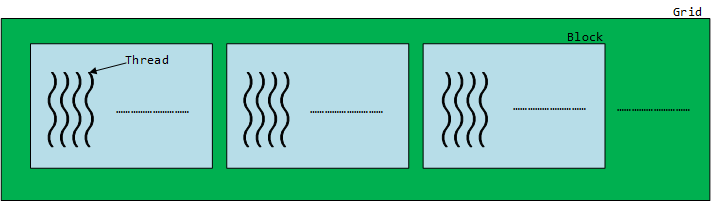
\includegraphics[width=\textwidth]{grid}

The dimensions of the grid and blocks are stated when the kernel is launched. The dimensions are called the \gls{execution configuration}. The example's execution configuration syntax was \verb|<<<2, 512>>>|. The first number is the number of blocks in the grid, which is the grid size. The second number is the number of threads per block, which is the block size. The product of the two gives the total number of threads in the grid. From a programming perspective, \verb|<<<1, 1024>>>| would give the same result. 1024 is also the typical limit of threads per block, but that depends on the compute capability of the device.

Within the kernel code, there are three API variables: threadIdx.x, blockIdx.x, and blockDim.x.\footnote{It is possible to have a 2D or 3D grid where threadIdx.y, threadIdx.z, and the like are used, but this paper will not use them}Using these variables, it's possible to find a unique ID for each thread. 

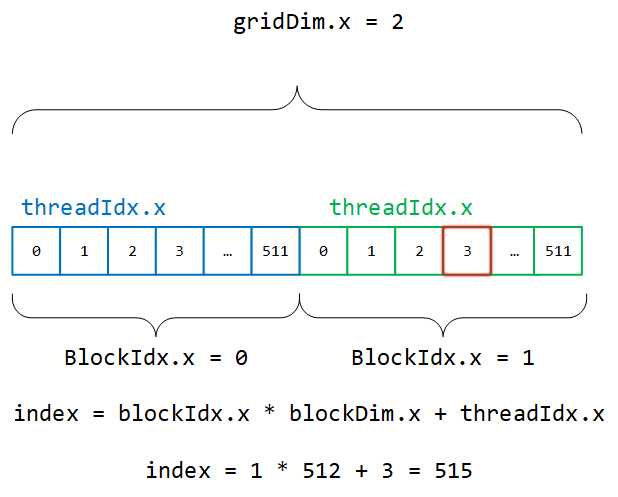
\includegraphics[width=0.95\textwidth]{img/cuda_indexing} 

This unique ID is typically used for indexing, as in my example.
\subsubsection{Hardware Perspective}
\indent From the hardware perspective, each GPU is a collection of memory and compute cores. There are CUDA cores which do arithmetic computations, also known as \glspl{sp}. There are also some special cores dedicated to specific purposes such as double precision operations, transcendental functions, the new Tensor cores for matrix multiplication, and the new raytracing cores. A collection of \glspl{sp} and these special cores make a \gls{sm}. Each \gls{sm}, alongside the cores, have shared memory, warp schedulders, L1 cache, and registers. On some devices, shared memory is physically the same as L1 cache. The entire GPU shares L2 cache, constant memory, and global memory.

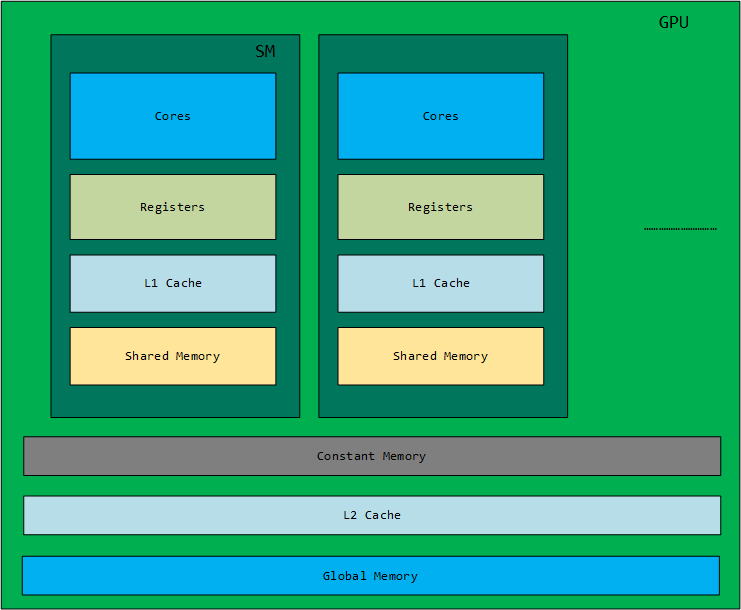
\includegraphics[width=0.95\textwidth]{hardware}

In order of fastest and smallest to slowest and largest, the memory hierarchy goes registers, shared memory, constant memory, and global memory.  This means that access to registers and shared memory is orders of magnitude faster than accessing global memory in terms of number of cycles. There are typically 64 K registers per \gls{sm}, 48 KB of shared memory, 64 KB of constant memory, and anywhere from 2-32GB of memory in global memory. These all depend on the device and the compute capability of the device.

\subsubsection{Where Hardware and Software Meet}
\indent Hardware and software interact through warps. A warp is a group of 32 threads. These 32 threads run in lock step, so each instruction in the 32 threads execute together. If there are less than 32 threads to execute, the warp will still run as if there were 32. Because of this, the number of threads per block should be a multiple of 32. If it's any less, then only a fraction of the warp is being utilized, and performance will take a massive hit. Each \gls{sm} has a specific number of warp schedulers depending on the compute capability of the device. Typically, this is four. \say{Then, at every instruction issue time each scheduler issues one instruction for one of its assigned warps, if any} \citep{cudaC}.

In an example, let's say that a \gls{sm} has 1024 threads running at the same time, which is typically the maximum number of threads per block. Each individual thread is not independent. 32 of them (a warp) are executed in lock step, with each assembly instruction being executed on the warp as a whole. This means that there are 32 warps. If the warps are distributed evenly across the four schedulers, each scheduler is assigned 8 warps. Each scheduler will execute a single lock instruction on one of these 8 warps on every single instruction cycle. Instruction cycles are typically every four clock cycles.The chosen warp becomes known as an active warp. The active warp is chosen purely based off available resources. If an instruction is waiting for memory to arrive from the global memory for 100 cycles, the warp scheduler will not call the next instruction on that particular warp until after those 100 cycles. An example order for the scheduler would be to execute instruction 10 on warp 0, then instruction 7 on warp 3, then instruction 2 on warp 6, then instruction 11 on warp 0. This continues for every instruction cycle as long as there are available resources for the warp, otherwise the scheduler has to wait. 

The amount of time that the schedulers have to wait will depend on the execution configuration(s) of the kernel(s) that are running. Ideally, every scheduler should be running an instruction every single instruction cycle. This is implicitly controlled by how the kernels access memory and how many warps and therefore threads there are per block.
\subsubsection{The Bottlenecks}
There are a several bottlenecks and caveats when programming for GPUs that will impede acceleration. These are the primary issues that I ran into.

\paragraph{Moving Data To/From the GPU} \hspace{0pt} \\
\indent The first issue is getting data on the chip in the first place. The CPU has to tell the memory to move data through the bus and into the \glspl{gpu} main, global memory. This can be done by calling two APIs to allocate memory and transfer memory to the device. Naturally, there is an API to free memory as well \citep{cudaC}.

\begin{minted}[breaklines, breakanywhere]{cuda}
    cudaResult_t cudaMalloc(void** ptr, size_t numberOfBytes);
    cudaResult_t cudaMemcpy(void* dst, void* src, cudaMemcpyKind kind, size_t numberOfBytes);
    cudaResult_t cudaFree(void* ptr);
\end{minted}

The bottleneck is the bus itself, whose transfer protocol is typically \gls{pcie}. GPUs are typically inserted into \gls{pcie} X16 slots on a desktop computer. This means that there are 16 lanes of data that can be transferred in parallel. The speed the different versions of \gls{pcie} are:
\begin{center}
PCIe Bandwidth
\begin{tabular}{ c c c}
Version Number & Bandwidth X1 & Bandwidth X16 \\
1.0 & 250 MB/s & 4 GB/s \\
2.0 & 500 MB/s & 8 GB/s \\
3.0 & 984.6 MB/s & ~15 GB/s \\
4.0 & 1969 MB/s & ~30 GB/s 
\end{tabular}

\citep{pci-sig}
\end{center}
Most motherboards nowadays use \gls{pcie} v3.0. For an example with \gls{pcie} v1.0, in an audio context, 4 GB is approximately an hour and a half of audio in stereo at 96kHz. This means that it will take at least 2 seconds to move the data back and forth - not even to process the data. The later versions of \gls{pcie} have faster bandwidth, but nowhere near close to the speed of the \gls{gpu}. This is why data sets should contain at least one million elements to make it worth \gls{gpu} acceleration. One million is a ballpark number peak where the CPU can computer faster than it takes for the data set to travel to and from the \gls{gpu}. For time domain convolution, my threshold number was 1024 elements. For frequency domain convolution, my threshold number was 8.3 million elements.

\paragraph{Global Memory Access} \hspace{0pt} \\
\indent The second issue comes after the data is on the \gls{gpu} chip. Global memory on the chip is anywhere from 2 GB to 32 GB. That's a worthwhile amount of memory, but the global memory is not directly connected to the cores. Global memory access is also the slowest type of memory access on a \gls{gpu}. This means that if all the threads need global memory access, there's a higher probability of the warp schedulers needing to wait for the memory to come to the cores. For example, a global memory access request may take 128 cycles to process. An instruction cycle is typically 4 cycles. Let's go back to the previous example where a SM has 1024 threads and 4 warp schedulers, so that there are 32 warps with 8 warps per scheduler. Lets say that instruction 1 is calculating the unique global ID: \verb|int threadID = blockIdx.x * blockDim.x + threadIdx.x|, instruction 2 is retrieving memory, and instruction 3 is incrementing the value. Let's also pretend that instruction 1 takes 8 cycles, or 2 instruction cycles. A single scheduler's instruction cycle could look like this:
\newpage
\begin{center}
Example Warp Scheduler Instruction Sequence
\begin{tabular}{ c c c}
 Instruction Cycle Number & Warp Number & Instruction Number\\ 
 1 & 0 & 1 \\  
 2 & 4 & 1 \\
 3 & 0 & 2 (must wait 32 cycles) \\
 4 & 7 & 1 \\
 5 & 2 & 1 \\
 6 & 4 & 2 (must wait 32 cycles) \\
 7 & 1 & 1 \\
 8 & 7 & 2 (must wait 32 cycles) \\
 9 & 3 & 1 \\
 10 & 2 & 2 (must wait 32 cycles) \\
 11 & 5 & 1 \\
 12 & 1 & 2 (must wait 32 cycles) \\
 13 & 3 & 2 (must wait 32 cycles) \\
 14 & 6 & 1 \\
 15 & 5 & 2 (must wait 32 cycles) \\
 16 & 6 & 2 (must wait 32 cycles) \\
 17 & waiting, no ready warps & \\
 18 & waiting, no ready warps & \\
 19 & waiting, no ready warps & \\
 20 & waiting, no ready warps & \\
 ......... & ......... & ......... \\
 35 & 0 & 3 \\
 36 & waiting, no ready warps & \\
 37 & waiting, no ready warps & \\
 38 & 4 & 3 \\
 39 & waiting, no ready warps & \\
 40 & 7 & 3 \\
 41 & waiting, no ready warps & \\
 42 & waiting, no ready warps & \\
 43 & waiting, no ready warps & \\
 44 & 1 & 3 \\
 45 & 3 & 3 \\
 46 & waiting, no ready warps & \\
 47 & 5 & 3 \\
 48 & 6 & 3
\end{tabular}
\end{center}

Half the instruction cycles are just waiting for data. This is far from ideal and is actually a 2x slowdown from the ideal. Because of this, there is a term called \gls{cgma}. This is a ratio of memory accesses to computations in a kernel. In my increment example, the \gls{cgma} was 1. The higher the \gls{cgma}, the better the performance \citep{kirk_hwu_2010}.

\subsubsection{Optimization Techniques}
\paragraph{Streams} \hspace{0pt} \\
\indent Streams are a software concept and \gls{cuda} \gls{api} for a queue of commands. In \gls{cuda}, streams are used to manage execution order and overlap of kernels and memory copies. By using streams, different tasks on the \gls{gpu} that would typically run sequentially can run in parallel. Streams can be created, synchronized, and destroyed throughout the program through these APIs \citep{cudaC}:
\begin{minted}[breaklines, breakanywhere]{cuda}
    cudaResult_t cudaStreamCreate(cudaStream_t* stream);
    cudaResult_t cudaStreamQuery(cudaStream_t stream);
    cudaResult_t cudaStreamSynchronize(cudaStream_t stream);
    cudaResult_t cudaStreamDestroy(cudaStream_t stream);
\end{minted}
The two most frequent applications of streams are for asynchronous memory copies and concurrent kernels. 
\subparagraph{Asynchronous Memory Copy} \hspace{0pt} \\
\indent Memory needs to be transferred from the host to the device, and this is one of the primary bottlenecks of \gls{gpu} computing, as detailed in the previous section. The API to transfer memory to the device is \citep{cudaC}:

\begin{minted}[breaklines, breakanywhere]{cuda}
    cudaResult_t cudaMemcpy(void** dst, void* src, cudaMemcpyKind kind,size_t numberOfBytes);
\end{minted}

This is an example of a synchronous API call, compared with an asynchronous API call. Synchronous means that it will prevent the program from progressing any further until this call has finished. Asynchronous means that control will return back to the host immediately after launch, allowing this task to finish in the meanwhile. There is an asynchronous flavor of \verb|cudaMemcpy()| \citep{cudaC}:

\begin{minted}[breaklines, breakanywhere]{cuda}
cudaResult_t cudaMemcpyAsync(void** dst, void* src, cudaMemcpyKind kind, size_t numberOfBytes, cudaStream_t stream);
\end{minted}
    
The caveat with asynchronous memory transfers is that it requires pinned memory. Pinned memory is an allocated section of RAM that can't be paged out to the disk. Pages are a virtual memory concept. Essentially, some processes have sections of memory that are stored on the disk to allow multiple processes to run independently, thinking that each has all of the physical memory available. Paging also allows the less frequently used memory to be stored in a location with larger capacity. The problem with pinned memory is that allocating too much of it will slow the process and all other processes running at the same time. Pinned memory is allocated and freed through CUDA APIs \citep{cudaC}:

\begin{minted}[breaklines, breakanywhere]{cuda}
    cudaResult_t cudaMallocHost(void** ptr, size_t numberOfBytes);
    cudaResult_t cudaFreeHost(void* ptr);
\end{minted}

My program combines synchronous and asynchronous memory transfers when moving the data to the device. Here is an abridged version of the code:

\begin{minted}[breaklines, breakanywhere]{cuda}
    cudaStream_t streams[4];
    float *d_ibuf, *ibuf;
    
    /*Open input file for reading*/
    SF_INFO i_info;
    SNDFILE *i_sndfile;
    i_sndfile = sf_open("input.wav", SFM_READ, &i_info);
	
	
    /*long long * iframes is defined as the size of the input
      long long * new_size is defined as pow(2, ceil(log2(N + K - 1)))
      checkCudaErrors(cudaResult_t) is an exception handler that will stop
        the program and print the error if an error occurs*/
    int mod = *iframes % 2;
    
    ...
    
    /*Allocate pinned memory*/
    checkCudaErrors(cudaMallocHost((void**)&ibuf, (*iframes / 2 + mod) * sizeof(float)));

    /*Allocate device memory*/
    checkCudaErrors(cudaMalloc(d_ibuf, *new_size * sizeof(float)));
    
    /*Create streams*/
    for(int i = 0; i < 4; i++){
        checkCudaErrors(cudaStreamCreate(&streams[i]));
	}
    
    ...
    
	/*Read in half of input*/
	sf_read_float(i_sndfile, ibuf, totalSize / 2);
	checkCudaErrors(cudaMemcpyAsync(*d_ibuf, ibuf, totalSize / 2 * sizeof(float), cudaMemcpyHostToDevice, streams[3]));

	...
	if(cudaStreamQuery(streams[3]) == cudaSuccess){
	    /*Read in other half of input*/
	    sf_read_float(i_sndfile, ibuf, totalSize / 2 + mod);
	    checkCudaErrors(cudaMemcpyAsync(*d_ibuf + totalSize / 2, ibuf, (totalSize / 2 + mod) * sizeof(float), cudaMemcpyHostToDevice, streams[3]));
	    ...
	    /*Do other things on the host*/
        ...
	}
	else{
	    ...
	    /*Do other things on the host*/
	    ...
	    /*Read in other half of input*/
	    sf_read_float(i_sndfile, ibuf, totalSize / 2 + mod);
	    checkCudaErrors(cudaMemcpyAsync(*d_ibuf + totalSize / 2, ibuf, (totalSize / 2 + mod) * sizeof(float), cudaMemcpyHostToDevice, streams[3]));
	}
	
\end{minted}

My code compromises between fully asynchronous memory transfers and a smaller pinned memory. I am expecting my input to grow very large, up to $2^{30}$ samples or $2^{32}$ bytes for my experiment, so I chose to only allocate half the amount of pinned memory required. Because of that, the first \verb|cudaMemcpy()| has to be synchronized before the second half of the audio can be read. Otherwise, the second call to \verb|sf_read_float| would overwrite the data while it's being transferred.

\subparagraph{Concurrent Kernels} \hspace{0pt} \\
\indent Another use for streams are for concurrent kernels. Kernel launches are asynchronous, but several kernel launches will proceed sequentially on the device. They do not run at the same time if called immediately after each other. Instead, the two kernels will be in a queue. Sometimes this is desired - for instance if two kernels affect the same data - and other times it is not, especially if the device is large enough to fit multiple grids. 

The number of concurrent kernels that can run on the device depends heavily on the compute capability, but it is typically 32. Other devices allow for 4, 16, and 128. Streams need to be created and added to the \gls{execution configuration} in order to allow concurrent kernels. 

\subparagraph{Full Example Of Streams} \hspace{0pt} \\
\begin{minted}[breaklines, breakanywhere]{cuda}
    /*input parameters that will get returned to the caller include 
      long long *iframes, long long *fframes, 
      float **d_ibuf, float **d_fbuf, 
      long long *new_size 
      
      input parameters given to this function include 
      const char *iname, const char *fname
      */
      
	cudaStream_t streams[4];
	float *ibuf, *fbuf;
	SF_INFO i_info, f_info;
	SNDFILE *i_sndfile, *f_sndfile;
	

	/*Read input*/
	i_sndfile = sf_open(iname, SFM_READ, &i_info);

	/*Read reverb*/
	f_sndfile = sf_open(fname, SFM_READ, &f_info);
	
	/*Store number of frames*/
	*iframes = i_info.frames;
	*fframes = f_info.frames;
	
	int mod = *iframes % 2;
	
	/*Find padded size for FFT*/
	*new_size = pow(2, ceil(log2((double)(*iframes + *fframes - 1))));
	
	/*Allocate device memory*/
	checkCudaErrors(cudaMalloc(d_ibuf, *new_size * sizeof(float)));
	checkCudaErrors(cudaMalloc(d_fbuf, *new_size * sizeof(float)));
	
	/*Allocate host pinned memory for input and filter*/
	checkCudaErrors(cudaMallocHost((void**)&ibuf, *iframes / 2 + mod * sizeof(float)));
	checkCudaErrors(cudaMallocHost((void**)&fbuf, *fframes * sizeof(float)));
	
	/*Create streams*/
	for(int i = 0; i < 4; i++){
		checkCudaErrors(cudaStreamCreate(&streams[i]));
	}
	
	/*Pad buffers with zeros*/
	/*FillWithZeros is a kernel that takes in a pointer, start element, and end element. All values from start to end become 0*/
	int numThreads = 512;
	int numBlocks = (*new_size - *fframes  + numThreads - 1) / numThreads;
	FillWithZeros<<<numBlocks, numThreads, 0, streams[0]>>>(*d_fbuf, *fframes,  *new_size);
	
	numBlocks = (*new_size - *iframes + numThreads - 1) / numThreads;
	FillWithZeros<<<numBlocks, numThreads, 0, streams[1]>>>(*d_ibuf, *iframes, *new_size);
	
	/*Read in half of input*/
	sf_read_float(i_sndfile, ibuf, totalSize / 2);
	checkCudaErrors(cudaMemcpyAsync(*d_ibuf, ibuf, totalSize / 2 * sizeof(float), cudaMemcpyHostToDevice, streams[3]));

	/*Read in all filter audio data*/
	sf_read_float(f_sndfile, fbuf, *fframes);

	/*Fill filter buffer*/
	checkCudaErrors(cudaMemcpyAsync(*d_fbuf, fbuf, *fframes * sizeof(float), cudaMemcpyHostToDevice, streams[2]));
	
	if(cudaStreamQuery(streams[3]) == cudaSuccess){
		/*Read in other half of input*/
		sf_read_float(i_sndfile, ibuf, totalSize / 2 + mod);
		checkCudaErrors(cudaMemcpyAsync(*d_ibuf + totalSize / 2, ibuf, (totalSize / 2 + mod) * sizeof(float), cudaMemcpyHostToDevice, streams[3]));
		checkCudaErrors(cudaStreamSynchronize(streams[2]));
		checkCudaErrors(cudaStreamDestroy(streams[2]));
		checkCudaErrors(cudaFreeHost(fbuf));
		sf_close(f_sndfile);
	}
	else{
		checkCudaErrors(cudaStreamSynchronize(streams[2]));
		checkCudaErrors(cudaStreamDestroy(streams[2]));
		checkCudaErrors(cudaFreeHost(fbuf));
		sf_close(f_sndfile);

		/*Read in other half of input*/
		checkCudaErrors(cudaStreamSynchronize(streams[3]));
		sf_read_float(i_sndfile, ibuf, totalSize / 2 + mod);
		checkCudaErrors(cudaMemcpyAsync(*d_ibuf + totalSize / 2, ibuf, (totalSize / 2 + mod) * sizeof(float), cudaMemcpyHostToDevice, streams[3]));		
	}
	/*Synchronize and destroy the rest of the streams*/
	for(int i = 0; i < 4; i++){
		if(i == 2) continue;
		checkCudaErrors(cudaStreamSynchronize(streams[i]));
		checkCudaErrors(cudaStreamDestroy(streams[i]));
	}	
	sf_close(i_sndfile);
	checkCudaErrors(cudaFreeHost(ibuf));
\end{minted}

Here, I have 4 streams, because there is a potential for 4 items to run concurrently: padding the filter with 0's, padding the input with 0's, copying the filter to the device, and copying the input to the device. Using streams, the program can hide the bottleneck of moving data to the \gls{gpu} by running \gls{cpu} functions at the same time.
\paragraph{Shared Memory} \hspace{0pt} \\
\indent In the past examples with streams and concurrent kernels, the third parameter of the execution configuration has been 0. That third parameter is actually to specify the amount of shared memory per block for each kernel. Shared memory, as discussed in the hardware perspective of \glspl{gpu}, is memory that is on each \gls{sm}. Because of this, accessing shared memory is significantly faster than accessing global memory. Shared memory can be declared statically inside the kernel such as \verb|__shared__ float x[512]| or dynamically in the third parameter of the execution configuration. Once declared, each thread in the block can load data into that shared memory at the same time and then use it. 

\begin{minted}[breaklines, breakanywhere]{cuda}
#define TILE 512
__global__ kernel(float *d_buf, int N){
    __shared__ data[TILE];
    int threadID = blockIdx.x * blockDim.x + threadIdx.x;
    
    if(threadID < N){
        data[threadIdx.x] = d_buf[threadID];
    }
    __syncthreads();
    
    /*Do some calculation with tile and store back in d_buf*/
}

... 
    /*N = size of d_buf*/
    int B = (N + TILE - 1) / TILE;
    kernel<<<B, TILE>>>(d_buf, N);
...
\end{minted}

\verb|__syncthreads()| is an API that will synchronize all of the threads in a block before proceeding. This barrier is there to make sure that \verb|data[]| is loaded with information before doing any calculations. I attempted to use shared memory for time domain convolution. However, this algorithm turned out to be less effective after timing tests.

\begin{minted}[breaklines, breakanywhere]{cuda}
#define tile 512
__global__ void timeDomainConvolutionExcessive(float *ibuf, float *fbuf, float *obuf, long long iFrames, int chunkNo){
	__shared__ float x[tile];
	__shared__ float h;
	
	if(chunkNo * tile + threadIdx.x < iFrames){
		x[threadIdx.x] = ibuf[chunkNo * tile + threadIdx.x];
	}
	h = fbuf[blockIdx.x];
		__syncthreads();
	if(chunkNo * tile + threadIdx.x < iFrames){
		atomicAdd(obuf + blockIdx.x + chunkNo * tile + threadIdx.x, x[threadIdx.x] * h);
	}
}
...
    /*main/caller*/
    int numChunks = (iFrames + tile - 1) / tile;
    cudaStream_t streams[numChunks];
    for(int i = 0; i < numChunks; i++){
        checkCudaErrors(cudaStreamCreate(&streams[i]));
        timeDomainConvolutionExcessive<<<fFrames, tile, 0, streams[i]>>>(d_ibuf, d_fbuf, d_obuf, iFrames, i);
    }
\end{minted}

\verb|atomicAdd()| takes in the address of what to add and the value to add that by. \verb|atomicAdd| prevents race conditions among different blocks by fusing the read, add, and write operations into a single instruction.

This algorithm is based off the cache-friendly time domain algorithm:
\begin{minted}[breaklines, breakanywhere]{cuda}
for k [0, K):
    for n [0, N):
        y[k + n] += x[n] * h[k]
\end{minted}
It divided the input into chunks of length \verb|tile|. There are \verb|fFrames| number of blocks, and each block corresponded to a point in the filter. 

This was an attempt to use shared memory, but it was ultimately not used because it was less accurate and slower. 
\paragraph{Memory Coalescing} \hspace{0pt} \\
\indent Memory coalescing builds off the concept of writing cache-friendly code, as discussed in the Sequential Time Domain Convolution section. Memory coalescing happens when the threads in a warp require sequential global memory access, such as threads 0 - 31 accessing elements 0 - 31 in an array of floats, respectively. The memory needs to be brought up from the global memory to L1 cache inside the \gls{sm}, and cache comes in blocks. An entire block of 128 bytes (32 elements if they are floats/ints) will be brought up from global memory to L1 cache. The best case scenario is that elements 0 - 31 land perfectly in this cache block. In that case, 32 global memory requests from a warp were \textit{coalesced} into a single global memory transaction. 

To try to coalesce global memory accesses, data should always be accessed sequentially among the threads. This will only happen with primitive data types like ints or floats. Structures might not land perfectly in the block since they contain primitive data types. This is known as alignment. The best case scenario is if access is aligned and also sequential. Otherwise, it will take at least two cache blocks to bring the 32 items. Memory allocated through \verb|cudaMalloc()| are guaranteed to be aligned to 256 bytes, so element 0, 32, 64, 96, etc of any array of floats is guaranteed to fall in the beginning of a cache block \citep{cudaCBestPractices}.

Memory coalescing is a tool and technique to help with the bottleneck of global memory access. It does complicate indexing within kernels. For instance, my kernel from above contained the line
\begin{minted}[breaklines, breakanywhere]{cuda}
atomicAdd(obuf + blockIdx.x + chunkNo * tile + threadIdx.x, x[threadIdx.x] * h);
\end{minted}

\verb|obuf + blockIdx.x + chunkNo * tile + threadIdx.x| is the entire line to calculate the position in the output that this thread is going to calculate. A visual cue to see if memory will be coalesced is to make sure that there is a \verb|+ threadIdx.x| and that \verb|threadIdx.x| is not multiplied by anything. That way, when threadIdx.x increments by one, the output pointer also increments by one. 

\paragraph{Scatter vs. Gather Decomposition} \hspace{0pt} \\
\indent For problems where the output requires multiple values of the input, such as time domain convolution, there are two ways to approach the problem. The first is a \say{gather-oriented approach} and the second is a \say{scatter-oriented approach} \citep{6216339}. The cache-unfriendly time domain convolution code is an example of a gather-oriented approach when the algorithm is parallelized:
\begin{minted}{cpp}
Gather Decomposition (Sequential)

for n [0, Y):
    value = 0
    for k [0, K):
        if (n - k < x.length):
            value += x[n - k] * h[k]
    n = value

\end{minted}
\begin{minted}[breaklines, breakanywhere]{cuda}
Gather Decomposition (Parallel)
__global__ void timeDomainConvolution(float *ibuf, float *fbuf, float *obuf, long long iFrames, long long fFrames){
    int threadID = blockIdx.x * blockDim.x + threadIdx.x;
    if(threadID < iFrames + fFrames - 1){
        float value = 0.0f;
        for(int k = 0; k < fFrames; k++){
            if (threadID - k > = 0 && threadID - k < iFrames){
                value += ibuf[threadID - k] * fbuf[k];
            }
        }
        obuf[threadID] = value;
    }
}
...
Eeach thread indexes an output element
\end{minted}
The cache-friendly algorithm for time domain convolution is considered a scatter decomposition.

\begin{minted}{cpp}
Scatter Decomposition (Sequential)
for k [0, K):
    for n [0, N):
        y[k + n] += x[n] * h[k]
\end{minted}
\begin{minted}[breaklines, breakanywhere]{cuda}
Scatter Decomposition (Parallel)
__global__ void timeDomainConvolutionAtomic(float *ibuf, float *fbuf, float *obuf, long long iFrames, long long fFrames){
    int threadID = blockIdx.x * blockDim.x + threadIdx.x;
	float h;
	if(threadID < fFrames){
		h = fbuf[threadID];
		for(int i = 0; i < iFrames; i++){
			atomicAdd(obuf + threadID  + i , ibuf[i] * h);
		}
	}
...
Each thread indexes a filter element
\end{minted}

Gather decompositions are better when parallelized because each thread writes to an independent output address. Scatter decompositions often suffer performance issues, because several threads write to the same output addresses. When multiple threads are writing to the same output address, there's a possibility of race conditions which will give unexpected answers. For instance, if two threads try to increment an address at the same exact time, the threads could write to their respective caches the new value. Then the value gets copied into main memory twice - resulting in only a single increment instead of two increments. \verb|atomicAdd()| ensures that the read, add, and write operations happen in one instruction so that another threads' read, add, and write operations will not interleave with the previous one. The problem with \verb|atomicAdd()| is that it will sequentialize parallel code. If several threads want to increment an address, \verb|atomicAdd()| forces them to queue, which will take a performance hit. 

For these two examples of algorithms, the gather decomposition is better even though memory is not necessarily being coalesced (in \verb|ibuf[threadID - k]|. \verb|fbuf[k]| is coalesced).
\subsection{CUDA Parellized Algorithms}
\subsubsection{Time Domain Convolution}
\paragraph{Algorithm Selection} \hspace{0pt} \\
\indent \par For time domain convolution, I tried four different algorithms with different optimization techniques which I labelled as: Atomic, Atomic Shared, Naive, and Excessive.

\begin{minted}[breaklines, breakanywhere]{cuda}
#define tile 512

__global__ void timeDomainConvolutionAtomic(float *ibuf, float *fbuf, float *obuf, long long iFrames, long long fFrames){
	int threadID = blockIdx.x * blockDim.x + threadIdx.x;
	float h;
	if(threadID < fFrames){
		h = fbuf[threadID];
		for(int i = 0; i < iFrames; i++){
			atomicAdd(obuf + threadID  + i , ibuf[i] * h);
		}
	}
	
}

__global__ void timeDomainConvolutionAtomicShared(float *ibuf, float *fbuf, float *obuf, long long iFrames, long long fFrames){
	__shared__ float x[tile];
	int threadID = blockIdx.x * blockDim.x + threadIdx.x;
	int numLoops = (iFrames + tile - 1) / tile;
	float h = 0.0f;
	if(threadID < fFrames){
		h = fbuf[threadID];
	}
	for(int n = 0; n < numLoops; n++){
		if(n * tile + threadIdx.x < iFrames){
			x[threadIdx.x] = ibuf[n * tile + threadIdx.x];
		}
		__syncthreads();
		for(int i = 0; i < tile; i++){
			if(n * tile + i < iFrames){
				atomicAdd(obuf + threadID + (n * tile) + i , x[i] * h);
			}
		}
		__syncthreads();
	}

}

__global__ void timeDomainConvolutionNaive(float *ibuf, float *fbuf, float *obuf, long long iframes, long long fFrames){
	int threadID = blockIdx.x * blockDim.x + threadIdx.x;
	if(threadID < iframes + fFrames - 1){
		int i_size = iframes;
		float value = 0;
		for(int k = 0; k < fFrames; k++){
			if(threadID - k >= 0 && threadID - k <= i_size){
				value += ibuf[threadID - k] * fbuf[k];
			}
		}
		obuf[threadID] = value;
	}
}

__global__ void timeDomainConvolutionExcessive(float *ibuf, float *fbuf, float *obuf, long long iFrames, int chunkNo){
	__shared__ float x[tile];
	__shared__ float h;
	
	if(chunkNo * tile + threadIdx.x < iFrames){
		x[threadIdx.x] = ibuf[chunkNo * tile + threadIdx.x];
	}
	h = fbuf[blockIdx.x];
	__syncthreads();
	if(chunkNo * tile + threadIdx.x < iFrames){
		atomicAdd(obuf + blockIdx.x + chunkNo * tile + threadIdx.x, x[threadIdx.x] * h);
	}
}
...
    /*ATOMIC*/
	numBlocks = (smallerFrames + numThreads - 1) / numThreads;
	timeDomainConvolutionAtomic<<< numBlocks, numThreads >>> (d_biggerBuf, d_smallerBuf, d_atomic, biggerFrames, smallerFrames);
	
	/*ATOMIC SHARED*/
	numBlocks = (smallerFrames + tile - 1) / tile;
	timeDomainConvolutionAtomicShared<<<numBlocks, tile >>>(d_biggerBuf, d_smallerBuf, d_atomic_shared, biggerFrames, smallerFrames);

	/*NAIVE*/
	numBlocks = (oFrames + numThreads - 1) / numThreads;
	timeDomainConvolutionPlain<<<numBlocks, numThreads >>>(d_biggerBuf, d_smallerBuf, d_naive, biggerFrames, smallerFrames);

	/*EXCESSIVE*/
	int numChunks = (biggerFrames + tile - 1) / tile;
	cudaStream_t streams[numChunks];
	for(int i = 0; i < numChunks; i++){
		checkCudaErrors(cudaStreamCreate(&streams[i]));
		timeDomainConvolutionExcessive<<<smallerFrames, tile, 0, streams[i]>>>(d_biggerBuf, d_smallerBuf, d_excessive, biggerFrames, i);
	}
...
\end{minted}

I lightly tested all of these and determined the accuracy of all of these algorithms based off a CPU-generated reference. In this test, K = 480,000 and N = 2,304,000. All trials were done on different \glspl{gpu}, but each trial was done on the same \gls{gpu}. 



For this experiment, the lower the time and smaller the accuracy, the better. So the naive algorithm is the winner. This is most likely do to the fact that the naive algorithm is the only gather decomposition algorithm. 
%\newpage
\begin{center}
Accuracy and Performance of Time Domain Convolution
\begin{tabular}{c c c c c}
 & Atomic & Atomic Shared & Naive & Excessive\\ 
 \textbf{TRIAL 1 }& & & \\
 Time (ms) & 61,269.718750 & 55,455.371094 &  19,140.958984 & 85,790.375000 \\  
 Accuracy & 3.981590E-05 & 5.722046E-05 & 2.622604E-06 & 1.606941E-04 \\
 \textbf{TRIAL 2} & & & \\
 Time (ms) & 37,341.425781  & 39,479.070312 & 7,031.311035 & 891,233.000000  \\
 Accuracy & 5.817413E-05 & 3.738447E+00 & 2.622604E-06 & 1.604557E-04 \\
 \textbf{TRIAL 3} & & & \\
 Time (ms) & 44,167.503906 & 46,413.277344 & 6,294.338867 & 747,803.625000 \\
 Accuracy & 4.386902E-05 & 3.738448E+00 & 2.622604E-06 & 1.602173E-04 \\
 \textbf{TRIAL 4} & & & \\
 Time (ms) & 53,322.039062 & 59,273.648438 & 11,514.409180 & 3,607,842.000000\\
 Accuracy & 5.626678E-05 & 3.886223E-05 & 2.622604E-06 & 1.604557E-04 \\
 \textbf{TRIAL 5} & & & \\
 Time (ms) & 62,557.585938 & 55,986.953125 & 19,912.279297 & 456,349.562500 \\
 Accuracy & 5.173683E-05 & 3.738460E+00 & 2.622604E-06 & 1.609325E-04 \\
 
\end{tabular}
\end{center}
\paragraph{Parallelized Peak Scaling} \hspace{0pt} \\
\indent For the finding the peak of the input and output, I used a library called Thrust. In Thrust, there is an API to find the extrema of an array \citep{thrust}.

\begin{minted}[breaklines, breakanywhere]{cuda}
__host__ __device__ thrust::pair<ForwardIterator,ForwardIterator> thrust::minmax_element(const thrust::detail::execution_policy_base< DerivedPolicy > &exec, ForwardIterator first, ForwardIterator last);
\end{minted}

This \gls{api} is called \verb|minmax_element()|. The first argument is either \verb|thrust::host| or \verb|thrust::device| depending on if the data is on the host or the device. These are special execution policies within Thrust. The second argument and third arguments are pointer wrappers to the first and last (exclusively last) element. The function returns a structure that contains two of these pointer wrappers, one for the minimum element and one for the maximum element in this array. Essentially, it takes in two addresses, scans all the values inbetween them, and returns two addresses. This is how I used it:
\begin{minted}[breaklines, breakanywhere]{cuda}

/*Functions to find extrema*/
float DExtrema(float *pointer, long long size){
	/*Convert raw float pointer into a thrust device pointer*/
	thrust::device_ptr<float> thrust_d_signal(pointer);
	
	thrust::pair < thrust::device_ptr<float>, thrust::device_ptr<float> >pair = thrust::minmax_element(thrust::device, thrust_d_signal, thrust_d_signal + size);
	float *d_min, *d_max;
	float min = 0, max = 0;
	
	d_min = pair.first.get();
	d_max = pair.second.get();
	
	checkCudaErrors(cudaMemcpy(&min, d_min, sizeof(float), cudaMemcpyDefault));
	checkCudaErrors(cudaMemcpy(&max, d_max, sizeof(float), cudaMemcpyDefault));

	return std::abs(min) > max ? std::abs(min) : max;
}


\end{minted}

I also have a kernel to scale all real numbers:

\begin{minted}[breaklines, breakanywhere]{cuda}

__global__ void RealFloatScale(float *a, long long size, float scale) {
	int numThreads = blockDim.x * gridDim.x;
	int threadID = blockIdx.x * blockDim.x + threadIdx.x;
	for (; threadID < size; threadID += numThreads) {
		a[threadID] *= scale;
	}
}
\end{minted}

\paragraph{Abridged Time Domain Convolution Code} \hspace{0pt} \\
\indent Put together, this is my abridged time domain convolution code, where \verb|**d_ibuf| is the input allocated on the device, and \verb|**d_fbuf| is the filter allocated on the device.
\begin{minted}[breaklines, breakanywhere]{cuda}
__global__ void timeDomainConvolutionNaive(float *ibuf, float *fbuf, float *obuf, long long iframes, long long fframes){
	int threadID = blockIdx.x * blockDim.x + threadIdx.x;
	if(threadID < iframes + fframes - 1){
		float value = 0;
		for(int k = 0; k < fframes; k++){
			if(threadID - k >= 0 && threadID - k <= fframes){
				value += ibuf[threadID - k] * fbuf[k];
			}
		}
		obuf[threadID] = value;
	}
}
float *TDconvolution(float ** d_ibuf, float ** d_fbuf, long long iFrames, long long oFrames){
    float *d_obuf, *obuf;
    long long fFrames = oFrames - iFrames + 1;

    /*Allocate device and host memory for the output*/
    checkCudaErrors(cudaMalloc(&d_obuf, oFrames * sizeof(float)));
    checkCudaErrors(cudaMallocHost((void**)&obuf, oFrames * sizeof(float)));

    /*Find peak of input*/
    float minmax = DExtrema(*d_ibuf, old_size);

    /*Launch the convolution  kernel*/
    int numThreads = 512;
    int numBlocks = (oFrames + numThreads - 1) /    numThreads;
    timeDomainConvolutionNaive<<<numBlocks, numThreads>>> (*d_ibuf, *d_fbuf, d_obuf, iFrames, fFrames);
    checkCudaErrors(cudaDeviceSynchronize());

    /*Find peak of output*/
    float minmax2 = DExtrema(d_obuf, oFrames);
    float scale = minmax/minmax2;

    /*Launch scaling kernel*/
    RealFloatScale <<< numBlocks, numThreads >>> (d_obuf, oFrames, scale);
    checkCudaErrors(cudaDeviceSynchronize());

    /* Copy device memory to host */
    checkCudaErrors(cudaMemcpy(obuf, d_obuf, oFrames * sizeof(float), cudaMemcpyDeviceToHost));

    checkCudaErrors(cudaFree(d_obuf));
    checkCudaErrors(cudaFree(*d_ibuf));
    checkCudaErrors(cudaFree(*d_fbuf));
    return obuf;
}
\end{minted}
\subsubsection{Frequency Domain Convolution}
\indent \par CUDA has an \gls{fft} library called cuFFT. The library was modeled after FFTW, and there is actually an interface to FFTW to allow people to easily port from FFTW to cuFFT. Just like in FFTW, there are \gls{fft} plans that need to be created, and there is an \gls{api} for R2C and C2R transforms to save time and memory capacity. The \glspl{api} look like this \citep{cufft}.

\begin{minted}[breaklines, breakanywhere]{cuda}
    cufftResult_t cufftCreate(cufftHandle* plan);
    cufftResult_t cufftPlan1d(cufftHandle* plan, int nx, cufftType type, int batch);
    cufftResult_t cufftExecR2C(cufftHandle plan, cufftReal *idata, cufftComplex *odata);
    cufftResult_t cufftExecC2R(cufftHandle plan, cufftComplex *idata, cufftReal *odata);
    cufftResult_t cufftDestroy(cufftHandle plan);
\end{minted}

These are incredibly similar to the FFTW plans. For the pointwise multiplication, there is a kernel with a modular function:

\begin{minted}[breaklines, breakanywhere]{cuda}
 __device__ __host__ inline Complex ComplexMul(Complex a, Complex b) {
	Complex c;
	c.x = a.x * b.x - a.y * b.y;
	c.y = a.x * b.y + a.y * b.x;
	return c;
}

__global__ void ComplexPointwiseMul(Complex *a, const Complex *b, int size) {
	const int numThreads = blockDim.x * gridDim.x;
	const int threadID = blockIdx.x * blockDim.x + threadIdx.x;
	for (int i = threadID; i < size; i += numThreads) {
		a[i] = ComplexMul(a[i], b[i]);
	}
}
\end{minted}

So the basic code looks like this: 

\begin{minted}[breaklines, breakanywhere]{cuda}
/*float **d_ibuf, float **d_fbuf, long long iFrames, long long fFrames, long long size are passed in*/
    
    /*Allocate memory for complex signal & filter*/

    /*Create FFT plans*/
    cufftHandle plan, outplan;
    CHECK_CUFFT_ERRORS(cufftPlan1d(&plan, size, CUFFT_R2C, 1));
    CHECK_CUFFT_ERRORS(cufftPlan1d(&outplan, size, CUFFT_C2R, 1));

    /*Transform Complex Signal*/
    CHECK_CUFFT_ERRORS(cufftExecR2C(plan, (cufftReal *) *d_ibuf, d_sig_complex));

    /*Transform Filter Signal*/
    CHECK_CUFFT_ERRORS(cufftExecR2C(plan, (cufftReal*) *d_fbuf, d_filter_complex));

    /*Convolution*/
    int blockSize = 256;
    int numBlocks = (size + blockSize - 1) / blockSize;
	
    ComplexPointwiseMul << < numBlocks, blockSize >> > (d_sig_complex, d_filter_complex, size / 2 + 1);

    /*IFFT*/
    CHECK_CUFFT_ERRORS(cufftExecC2R(outplan, d_sig_complex, *d_ibuf));
    
    /*Scale the output according to the input*/
    /*Copy to host*/
    /*Cleanup memory*/
\end{minted}
\paragraph{cuFFT Callback Routine} \hspace{0pt} \\
\indent There is a special \gls{api} in the cuFFT library that allows for functions to modify the data before and/or after a transform, and it is embedded within the transform. These are custom cuFFT callbacks. According to NVIDIA, larger input sizes can improve performance by 20\% \citep{cufft_callbacks}. Modifying the data before the transform is known as a load callback, and modifying the data after the transform is known as a store callback. cuFFT supports several different types of transforms, so there are a total of 8 different callback types. 

Convolution can utilize a load callback into the inverse, C2R. The load callback will modify complex data on a point-by-point basis before sending it to the C2R. This is function prototype for the load callback \citep{cufft}.

\begin{minted}[breaklines, breakanywhere]{cuda}
    typedef cufftComplex (*cufftCallbackLoadC)(void *dataIn, size_t offset, void *callerInfo, void *sharedPointer);
\end{minted}

A callback needs to be defined, and then a device pointer to the callback routine must be defined. The host then must copy this device pointer and pass it to cuFFT. The setup syntax looks like this:
\begin{minted}[breaklines, breakanywhere]{cuda}
    /*Declarations/Definitions*/
    __device__ __host__ inline Complex ComplexMul(Complex a, Complex b) {
    	Complex c;
    	c.x = a.x * b.x - a.y * b.y;
    	c.y = a.x * b.y + a.y * b.x;
    	return c;
    }
    __device__ cufftComplex cbComplexPointwiseMul(void *dataIn, size_t offset, void *cb_info, void *sharedmem) {
	    cufftComplex *filter = (cufftComplex*)cb_info;
	    return (cufftComplex) ComplexMul(((Complex *)dataIn)[offset], filter[offset]);
	}
	
    // Define the device pointer to the callback routine. 
    __device__ cufftCallbackLoadC myOwnCallbackPtr = cbComplexPointwiseMul;
\end{minted}

This means that I don't have to use the complex multiplication kernel explicitly. The convolution section of the code with the callback looks like this:

\begin{minted}[breaklines, breakanywhere]{cuda}
    /*float **d_ibuf, float **d_fbuf, long long iFrames, long long fFrames, long long size are passed in*/
    
    /*Allocate memory for complex signal & filter*/
    
    /*Create FFT plans*/
    cufftHandle plan, outplan;
    CHECK_CUFFT_ERRORS(cufftPlan1d(&plan, size, CUFFT_R2C, 1));
    CHECK_CUFFT_ERRORS(cufftPlan1d(&outplan, size, CUFFT_C2R, 1));
	
    /*Transform Signals*/
    CHECK_CUFFT_ERRORS(cufftExecR2C(plan, (cufftReal *)*d_ibuf, d_sig_complex));
    CHECK_CUFFT_ERRORS(cufftExecR2C(plan, (cufftReal*)*d_fbuf, d_filter_complex));
	
    /*Copy over the host copy of callback function*/
    cufftCallbackLoadC hostCopyOfCallbackPtr;
    checkCudaErrors(cudaMemcpyFromSymbol(&hostCopyOfCallbackPtr,myOwnCallbackPtr, sizeof(hostCopyOfCallbackPtr)));
	
    /*Associate the load callback with the plan*/
    CHECK_CUFFT_ERRORS(cufftXtSetCallback(outplan, (void **)&hostCopyOfCallbackPtr, CUFFT_CB_LD_COMPLEX, (void **)&d_filter_complex));

    /*Transform signal back, callback pointwise multiplies on the way in*/
    CHECK_CUFFT_ERRORS(cufftExecC2R(outplan, d_sig_complex, *d_ibuf));
	
    /*Scale the output according to the input*/
    /*Copy to host*/
    /*Cleanup memory*/
\end{minted}
\paragraph{In-Place Overlap-Add within one GPU} \hspace{0pt} \\
\indent Frequency domain convolution takes up extra memory to account for the complex arrays. cuFFT itself needs some spare scratch space called a workspace to be able to do the computations. Because of this, the input could be too big to fit on the \gls{gpu}. To account for that, the input can be divided into chunks and convolved chunk by chunk, as described earlier. To make sure that we don't run out of space, we can do in-place overlap-add. The algorithm is the same as detailed in the Sequential Frequency Domain section, but in-place adds more steps.

To find the block amount ($M + L$), I use a few \glspl{api}. Whatever the block size is, there will be four arrays of that size in bytes - two for complex and two for real. So the total amount of memory to allocate will approximately be \verb|blockSize * 16|. There's a couple memory \glspl{api} that I used to calculate the maximum size of the block that will fit on the device \citep{cufft}, \citep{cudaC}.

\begin{minted}[breaklines, breakanywhere]{cuda}
    cufftResult cufftEstimate1d(int nx, cufftType type, int batch, size_t *workSize);
    cudaResult_t cudaMemGetInfo(size_t *free, size_t *total);
\end{minted}

\verb|cufftEstimate1d()| fills workSize with the amount of space it should take to perform the transform. \verb|cudaMemGetInfo()| returns the amount of free and total global memory left on the device. To find the maximum size of the block that will fit on the device, I used a loop and overestimated the amount of bytes to be 18x the block size instead of 16:

\begin{minted}[breaklines, breakanywhere]{cuda}
int myExp = ceil(log2((float)(iFrames + M)));
size_t blockSize = pow(2, myExp);
int L = iFrames, blockNum = 0;
size_t workspace;
CHECK_CUFFT_ERRORS(cufftEstimate1d(blockSize, CUFFT_R2C, 2, &workspace));
while(getFreeSize() < workspace + blockSize * 18L){
	myExp--;
	blockSize = pow(2, myExp);
	blockNum++;
	CHECK_CUFFT_ERRORS(cufftEstimate1d(blockSize, CUFFT_R2C, 2, &workspace));
}
\end{minted}

This is what the in-place algorithm looks like, along with matching code.

\def\excerpt{\thispagestyle{empty} \paragraph{In-Place Overlap-Add Algorithm} \hspace{0pt} \\}
\includepdf[pages=5, scale=0.95,
pagecommand={\excerpt}]{Algorithms.pdf}

\begin{minted}[breaklines, breakanywhere]{cuda}
/*Memory has been allocated, number of blocks has been determined*/
/*Callback function has been set and attached to outplan*/
/*Filter has already been transformed above*/
for(int blockNo = 0; blockNo <= blockNum; blockNo++){
	long long cpyAmount = L;
	if (blockNo == blockNum) {
		cpyAmount = iFrames % L;
	}
	checkCudaErrors(cudaMemcpy(d_padded_signal, &d_obuf[L * blockNo], cpyAmount * sizeof(float), cudaMemcpyDeviceToDevice));
	
	if (blockNo != 0) {
		checkCudaErrors(cudaMemcpy(&d_obuf[L * blockNo], &d_padded_signal[L], M * sizeof(float), cudaMemcpyDeviceToDevice));
	}
	
	/*fillWithZeroes is a wrapper to a thrust API to fill with 0's. Params: (array, start, end)*/
	fillWithZeroes(&d_padded_signal, cpyAmount, blockSize);
	
	/*Transform signal*/
	CHECK_CUFFT_ERRORS(cufftExecR2C(plan, (cufftReal *)d_padded_signal, d_sig_complex));

	/*IFFT*/
	CHECK_CUFFT_ERRORS(cufftExecC2R(outplan, d_sig_complex, d_padded_signal));
	if (blockNo != 0) {
		PointwiseAdd << <numBlocks, numThreads >> > (d_padded_signal, &d_obuf[blockNo * L], M);
	}
	
	/*Initial case*/
	if (blockNo == 0) {
	    checkCudaErrors(cudaMemcpy(d_obuf, d_padded_signal, L * sizeof(float), cudaMemcpyDeviceToDevice));
	}
	/*Last case*/
	else if (blockNo == blockNum) {
		checkCudaErrors(cudaMemcpy(&d_obuf[blockNo * L + M], &d_padded_signal[M], cpyAmount * sizeof(float), cudaMemcpyDeviceToDevice));
	}
        /*Every other case*/
        else{
		checkCudaErrors(cudaMemcpy(&d_obuf[blockNo * L + M], &d_padded_signal[M], (L - M) * sizeof(float), cudaMemcpyDeviceToDevice));
	}
}
\end{minted}
\paragraph{Overlap-Add with multiple GPUs} \hspace{0pt} \\
\indent This same concept of overlap-add can be used on multiple \glspl{gpu} instead of just one. Several servers have multiple cards, and they can be accessed in CUDA code individually. This way, all asynchronous calls will run at the same time. This is used through \verb|cudaSetDevice(int devNum)|. 

The approach I used is to find out the largest block that can fit on each card and fill each one until there are no more input samples left to distribute. This would involve finding the amount of free space on the card and dividing by a the number of bytes I plan to allocate (plus more to be conservative and prevent allocation errors). Once the largest size that can fit on the device is discovered, subtract $K-1$ to find the amount of input samples that can be convolved on the device. This does not distribute the input evenly, and there is a potential that all the cards are not being used. I had an array called \verb|size_t inSizes[numDevices]| where I stored the block sizes for each device.

\begin{minted}[breaklines, breakanywhere]{cuda}
/*numDevs = number of devices
getFreeSize() returns the free amount in global memory on the device
size_t inSizes[] is an array to store the block size per device
d_ibufs is the input array
iFrames = input size
M = fFrames - 1
*/
size_t freeSizes[numDevs];
/*Find out amount of free memory on each device*/
for (int i = 0; i < numDevs; i++) {
    cudaSetDevice(i);
    freeSizes[i] = getFreeSize();
    /*most precise is input = freeSize()/16 - 16, but dividing by 32 to conservatively account for cuFFT space*/
    size_t freeSize = freeSizes[i] / 32;
    /*max number of elements that's a power of 2*/
    inSizes[i] = pow(2, floor(log2((double)freeSize)));
}
/*Allocate the block amount, stop if we've used all of the input*/
long long frames = 0;
for(int i = 0; i < numDevs; i++){
    cudaSetDevice(i);
    if(frames >= iFrames){
        inSizes[i] = 0;
        continue;
    }
    frames += inSizes[i] - M;
    checkCudaErrors(cudaMalloc(&d_ibufs[i], inSizes[i] * sizeof(float)));
    checkCudaErrors(cudaMalloc(&d_rbufs[i], inSizes[i] * sizeof(float)));
    checkCudaErrors(cudaMalloc(&d_Cbufs[i], (inSizes[i] + 2) * sizeof(cufftComplex)));
}
/*Copy memory to devices and pad with zeros. Do the 4 tasks in 4 different streams per device*/
int streamsPerDev = 4;
cudaStream_t stream[numDevs * streamsPerDev];
for(int i = 0; i < numDevs; i++){
    cudaSetDevice(i);
    checkCudaErrors(cudaStreamCreate(&stream[i * streamsPerDev]));
    checkCudaErrors(cudaStreamCreate(&stream[i * streamsPerDev + 1]));
    checkCudaErrors(cudaStreamCreate(&stream[i * streamsPerDev + 2]));
    checkCudaErrors(cudaStreamCreate(&stream[i * streamsPerDev + 3]));
    if (inSizes[i] == 0){
        continue;
    }
    long long amtRead = inSizes[i] - M;
    if (frames + amtRead > iFrames){
        amtRead = iFrames - frames;
    }
    checkCudaErrors(cudaMemcpyAsync(d_ibufs[i], ibuf + frames, amtRead * sizeof(float), cudaMemcpyHostToDevice, stream[i * streamsPerDev]));
    numBlocks = (inSizes[i] - amtRead + blockSize - 1 ) / blockSize;
    FillWithZeros<<<numBlocks, blockSize, 0, stream[i * streamsPerDev + 1]>>>(d_ibufs[i], amtRead, inSizes[i]);
    numBlocks = (inSizes[i] - rFrames - 1 + blockSize) / blockSize;
    FillWithZeros<<<numBlocks, blockSize, 0, stream[i * streamsPerDev + 2]>>>(d_rbufs[i], rFrames, inSizes[i]);
    checkCudaErrors(cudaMemcpyAsync(d_rbufs[i], rbuf, rFrames * sizeof(float), cudaMemcpyHostToDevice, stream[i * streamsPerDev + 3]));
    frames += amtRead;
}
\end{minted}

\paragraph{Multi-GPU + Block Convolution} \hspace{0pt} \\
\indent There's a possibility that the input data will be so large that it can't fit on all of the \glspl{gpu}. This is because cuFFT requires extra global memory in order to compute the transform, which is why I divided the free space by 32. If that happens, I find out if all the \glspl{gpu} contain enough memory to at least fit the input signal and the filter. In addition, the device with the largest amount of memory should contain the output buffer. If these conditions are not met, then end the program gracefully.

\begin{minted}[breaklines, breakanywhere]{cuda}
for (int i = 0; i < numDevs; i++) {
	cudaSetDevice(i);
	freeSizes[i] = getFreeSize();
	/*most precise is input = freeSize()/16 - 16, but dividing by 32 to conservatively account for cuFFT space*/
	size_t freeSize = freeSizes[i] / 32;
	/*max number of elements that's a power of 2*/
	inSizes[i] = pow(2, floor(log2((double)freeSize)));
}
long long totalAllowedFrames = 0;
for(int i = 0; i < numDevs; i++){
	totalAllowedFrames += inSizes[i] - M;
}
long long frames = 0;
if (totalAllowedFrames > iFrames){
	/*Do single block convolution & allocate memory for normal case*/
}
else{
    doubleBlock = true;
    /*Verifying total memory on all GPUs*/
	totalAllowedFrames = 0;
	for(int i = 0; i < numDevs; i++){
		/*Theoretically should be 4. Dividing by 8 to be conservative*/
		totalAllowedFrames += freeSizes[i] / 4;
		totalAllowedFrames -= rFrames;
		if (maxFree < freeSizes[i]){
			maxFree = freeSizes[i];
			singleDev = i;
		}
	}
	if(totalAllowedFrames < iFrames + M * numDevs || 
		freeSizes[singleDev] / 4 - inSizes[singleDev] < oFrames + M){
		fprintf(stderr, "\n\nERROR: NOT ENOUGH COLLECTIVE MEMORY ON THE GPUs. EXITING\n\n");
		checkCudaErrors(cudaFreeHost(ibuf));
		free(rbuf);
		return NULL;
	}
	...
\end{minted}

Otherwise, if there is enough collective memory on all of the devices, begin by trying to divide the input evenly among the devices. If there are 4 cards, then give $\ceil{\frac{N}{4}}$ to each card. If however, the amount of available memory on one card will not fit $\ceil{\frac{N}{4}}$, then distribute the memory like before - fill every card up completely until there is no more input left.

\begin{minted}[breaklines, breakanywhere]{cuda}
/*Check to see if input can divide evenly, or if we fill each up to the brim*/
amtPerDevice = (iFrames + numDevs - 1) / numDevs;
for(int i = 0; i < numDevs; i++){
    /*Theoretically should be 4. Dividing by 8 to be conservative*/
    size_t freeSize = freeSizes[i] / 8 - rFrames;
    freeSize = pow(2, floor(log2((double)freeSize)));
    if (amtPerDevice + M > freeSize){
        fprintf(stderr, "WARNING: One GPU doesn't have enough memory to divide evenly. Redistributing memory.\n");
        amtPerDevice = iFrames;
        break;
    }
}
		
long long framecount = 0;
for(int i = 0; i < numDevs; i++){
	cudaSetDevice(i);
	/*Theoretically should be 4. Dividing by 8 to be conservative*/
	size_t freeSize = freeSizes[i] / 8;
	freeSize -= rFrames;
	freeSize = pow(2, floor(log2((double)freeSize)));
	int currFrames = amtPerDevice;
	if (currFrames + M > freeSize){
	    currFrames = freeSize - M;
	}
	if(framecount + currFrames > iFrames){
		currFrames = iFrames - framecount;
	}
	if(currFrames == 0){
		inSizes[i] = 0;
		continue;
	}
	inSizes[i] = currFrames + M;
	checkCudaErrors(cudaMalloc(&d_ibufs[i], inSizes[i] * sizeof(float)));
	checkCudaErrors(cudaMalloc(&d_rbufs[i], rFrames * sizeof(float)));
	framecount += currFrames;
}
/*Verify that all of the input was split among all the GPUs*/
if(framecount < iFrames){
    fprintf(stderr, "\n\nERROR: NOT ENOUGH COLLECTIVE MEMORY ON THE GPUs. EXITING\n\n");
	checkCudaErrors(cudaFreeHost(ibuf));
	for(int i = 0; i < numDevs; i++){
		cudaSetDevice(i);
		checkCudaErrors(cudaFree(d_ibufs[i]));
		checkCudaErrors(cudaFree(d_rbufs[i]));
	}
	free(rbuf);
	return NULL;
}
\end{minted}

Then, instead of running a simple convolution, I run a block convolution inside each \gls{gpu}, basing the size of the block off \verb|cufftEstimate1d()| as previously stated in the block convolution for a single \gls{gpu}. In addition, the memory copy will be slightly different.

\begin{minted}[breaklines, breakanywhere]{cuda}
frames = 0;
for(int i = 0; i < numDevs; i++){
	cudaSetDevice(i);
	/*Create 4 streams*/
	if (inSizes[i] == 0) continue;
	long long amtRead = inSizes[i] - M;
	if (frames + amtRead > iFrames){
		amtRead = iFrames - frames;
	}
	checkCudaErrors(cudaMemcpyAsync(d_ibufs[i], ibuf + frames, amtRead * sizeof(float), cudaMemcpyHostToDevice, stream[i * streamsPerDev]));
	numBlocks = (inSizes[i] - amtRead + blockSize - 1 ) / blockSize;
	FillWithZeros<<<numBlocks, blockSize, 0, stream[i * streamsPerDev + 1]>>>(d_ibufs[i], amtRead, inSizes[i]);
	if(!doubleBlock){	
		numBlocks = (inSizes[i] - rFrames - 1 + blockSize) / blockSize;
		FillWithZeros<<<numBlocks, blockSize, 0, stream[i * streamsPerDev + 2]>>>(d_rbufs[i], rFrames, inSizes[i]);
	}
	checkCudaErrors(cudaMemcpyAsync(d_rbufs[i], rbuf, rFrames * sizeof(float), cudaMemcpyHostToDevice, stream[i * streamsPerDev + 3]));
	frames += amtRead;
}
\end{minted}
\indent \par My full source code can be found in the appendix.

\subsection{Results}

\subsubsection{Preparation and Inputs}
\indent \par My input data set consists of 26 different sized inputs and one filter. The inputs sizes were $2^4$, $2^5$, $2^6$, ... $2^{30}$ samples long. For preparation, I created sine sweeps/chirps of that many samples long using Erik D Castro Lopo's sndfile-tools, and I exported them into mono wave files at 96kHz \citep{lopo_2017}. My filter was 480,000 samples, which is equivalent to 5 seconds of audio at 96kHz.

I used the New York University High Performance Computing (NYU HPC) clusters for my benchmarking tests\footnote{www.nyu.edu/life/information-technology/research-and-data-support/high-performance-computing.html}. I also used the Courant Institute of Mathematical Sciences (CIMS) GPU Computing servers\footnote{cims.nyu.edu/webapps/content/systems/resources/computeservers} for preliminary testing and profiling. The \glspl{gpu} that I have tested on at the NYU HPC are Tesla K80 (4/8 per node), Geforce GTX 1080 (4 per node), Tesla P40 (4 per node), Tesla P100(4 per node), and Tesla V100 (2/4 per node). CIMS servers have two Geforce GTX TITAN Black on one server, GeForce GTX TITAN Z and two GeForce GTX Titan X on another, and two GeForce GTX Titan Z on the last. 

In terms of \glspl{cpu}, I used the same compute clusters. The NYU HPC has several types and generations of CPUs including codename IvyBridge, Broadwell, Haswell, and Skylake, and they all have different processor speeds. The exact CPU I used will be specified in the charts. The CIMS servers have AMD Opterons (6272 and 6136), which I did preliminary testing on.

I did 10 trials of the same input set for \gls{gpu} time domain convolution, \gls{gpu} frequency domain convolution, and \gls{cpu} frequency domain convolution. Unfortunately, \gls{cpu} time domain convolution took too long. Input sizes of $2^{29}$ and $2^{30}$ took too long to complete on the \gls{hpc} clusers that I was using. I also only did one trial for $2^4 - 2^{28}$ in the time domain because the later inputs took so much time. $2^{29}$ is projected to take 9 days, and $2^{30}$ is projected to take 19 days to compute for Sequential Time Domain Convolution. 

All \gls{gpu} results had an accuracy of at least $1 \cdot 10^{-5}$ in comparison to the \gls{cpu}. The largest inaccuracies were around $2 \cdot 10^{-6}$.

\subsubsection{Average Results}
    \includegraphics[width=\textwidth]{"Time Domain Convolution CPU vs GPU"}
    \includegraphics[width=\textwidth]{"Time Domain Convolution CPU vs GPU (1)"}
    
    \includegraphics[width=\textwidth]{"Frequency Domain Convolution CPU vs GPU"}
    \includegraphics[width=\textwidth]{"Frequency Domain Convolution CPU vs GPU (1)"}
    
    \includegraphics[width=\textwidth]{"Convolve Time CPU vs GPU"}
\begin{center}
    Intel(R) IvyBridge @ 3.00GHz with 62 / 188 GB memory
    
    Time For CPU Time Domain Convolution
    
    \begin{tabular}{c | c | c | c}
         Input Size & Time (s) &  Approximate Computation Time (s) & Percentage Computation Time \\
        $2^4$ & 0.198 & 0.030 & 15.15\% \\
        $2^5$ & 0.062 & 0.050 & 80.65\% \\
        $2^6$ & 0.129 & 0.100 & 77.52\% \\
        $2^7$ & 0.207 & 0.200 & 96.62\% \\
        $2^8$ & 0.401 & 0.390 & 97.26\% \\
        $2^9$ & 0.791 & 0.780 & 98.61\% \\
        $2^{10}$ & 1.568 & 1.560 & 99.49\% \\
        $2^{11}$ & 3.132 & 3.110 & 99.30\% \\
        $2^{12}$ & 6.245 & 6.230 & 99.76\% \\
        $2^{13}$ & 12.462 & 12.440 & 99.82\% \\
        $2^{14}$ & 24.928 & 24.890 & 99.85\% \\
        $2^{15}$ & 49.790 & 49.740 & 99.90\% \\
        $2^{16}$ & 99.584 & 99.460 & 99.88\% \\
        $2^{17}$ & 199.248 & 199.150 & 99.95\% \\
        $2^{18}$ & 398.551 & 398.130 & 99.89\% \\
        $2^{19}$ & 796.193 & 795.980 & 99.97\% \\
        $2^{20}$ & 1592.686 & 1592.060 & 99.96\% \\
        $2^{21}$ & 3199.540 & 3198.720 & 99.97\% \\
        $2^{22}$ & 6436.107 & 6435.200 & 99.99\% \\
        $2^{23}$ & 12855.971 & 12854.270 & 99.99\% \\
        $2^{24}$ & 25759.761 & 25751.890 & 99.97\% \\
        $2^{25}$ & 51318.888 & 51296.400 & 99.96\% \\
        $2^{26}$ & 102916.184 & 102798.050 & 99.89\% \\
        $2^{27}$ & 205237.316 & 205057.440 & 99.91\% \\
        $2^{28}$ & 412070.139 & 411756.310 & 99.92\% \\
    \end{tabular} 
    \newpage
    
    1 Tesla P40, 24 GB Memory
    
    Average Time For GPU Time Domain Convolution
    
    \begin{tabular}{c | c | c | c}
         Input Size & Average Time (s) &  Approximate Computation Time (s) & Percentage Computation Time \\
         $2^4$ & 1.9813 & 0.003018096 & 0.15\% \\
         $2^5$ & 1.9313 & 0.0047808736 & 0.25\% \\
         $2^6$ & 1.9252 & 0.0051817632 & 0.27\% \\
         $2^7$ & 1.9288 & 0.0054029632 & 0.28\% \\
         $2^8$ & 1.9179 & 0.0064762464 & 0.34\% \\
         $2^9$ & 1.9268 & 0.0073473792 & 0.38\% \\
         $2^{10}$ & 1.9323 & 0.0097226944 & 0.50\% \\
         $2^{11}$ & 1.9258 & 0.013106544 & 0.68\% \\
         $2^{12}$ & 1.935 & 0.0207268895 & 1.07\% \\
         $2^{13}$ & 1.9413 & 0.0355993409 & 1.83\% \\
         $2^{14}$ & 1.9824 & 0.0647762336 & 3.27\% \\
         $2^{15}$ & 2.0446 & 0.1231666786 & 6.02\% \\
         $2^{16}$ & 2.1249 & 0.2105333726 & 9.91\% \\
         $2^{17}$ & 2.3295 & 0.4084287079 & 17.53\% \\
         $2^{18}$ & 2.7978 & 0.8491014223 & 30.35\% \\
         $2^{19}$ & 3.6862 & 1.762778601 & 47.82\% \\
         $2^{20}$ & 5.2535 & 3.312563647 & 63.05\% \\
         $2^{21}$ & 8.3561 & 6.420397461 & 76.83\% \\
         $2^{22}$ & 14.6672 & 12.63506641 & 86.15\% \\
         $2^{23}$ & 27.0572 & 25.09269219 & 92.74\% \\
         $2^{24}$ & 51.9975 & 49.99425547 & 96.15\% \\
         $2^{25}$ & 101.7667 & 99.69218125 & 97.96\% \\
         $2^{26}$ & 201.1397 & 198.9340703 & 98.90\% \\
         $2^{27}$ & 400.7261 & 398.3048813 & 99.40\% \\
         $2^{28}$ & 797.9594 & 795.079025 & 99.64\% \\
         $2^{29}$ & 1597.2998 & 1593.526625 & 99.76\% \\
         $2^{30}$ & 3195.1222 & 3189.6074 & 99.83\% 
    \end{tabular}
    \newpage
    Time Domain Speedup Amount
    
     \begin{tabular}{c | c}
         Input Size & Speedup amount (CPU time / GPU time) \\
$2^4$ & 0.0999 \\
$2^5$ & 0.0321 \\
$2^6$ & 0.067 \\
$2^7$ & 0.1073 \\
$2^8$ & 0.2091 \\
$2^9$ & 0.4105 \\
$2^{10}$ & 0.8115 \\
$2^{11}$ & 1.6263 \\
$2^{12}$ & 3.2274 \\
$2^{13}$ & 6.4194 \\
$2^{14}$ & 12.5747 \\
$2^{15}$ & 24.352 \\
$2^{16}$ & 46.8653 \\
$2^{17}$ & 85.5325 \\
$2^{18}$ & 142.4516 \\
$2^{19}$ & 215.9929 \\
$2^{20}$ & 303.1667 \\
$2^{21}$ & 382.8987 \\
$2^{22}$ & 438.8095 \\
$2^{23}$ & 475.1405 \\
$2^{24}$ & 495.4038 \\
$2^{25}$ & 504.2798 \\
$2^{26}$ & 511.6652 \\
$2^{27}$ & 512.1636 \\
$2^{28}$ & 516.4049
    \end{tabular}
    \newpage
    Intel(R) IvyBridge @ 3.00GHz, 1510 GB Memory
    
    Average Time For CPU Frequency Domain Convolution
   
    \begin{tabular}{ c | c | c | c }
        Input Size & Wall-Clock Time (s) &  Approximate Computation Time (s) & Percentage Computation Time \\
$2^{4}$ & 0.066 & 0.042 & 63.64\% \\
$2^{5}$ & 0.054 & 0.04 & 74.07\% \\
$2^{6}$ & 0.054 & 0.041 & 75.93\% \\
$2^{7}$ & 0.054 & 0.041 & 75.93\% \\
$2^{8}$ & 0.053 & 0.04 & 75.47\% \\
$2^{9}$ & 0.053 & 0.037 & 69.81\% \\
$2^{10}$ & 0.052 & 0.039 & 75.00\% \\
$2^{11}$ & 0.055 & 0.041 & 74.55\% \\
$2^{12}$ & 0.052 & 0.039 & 75.00\% \\
$2^{13}$ & 0.054 & 0.041 & 75.93\% \\
$2^{14}$ & 0.054 & 0.041 & 75.93\% \\
$2^{15}$ & 0.058 & 0.038 & 65.52\% \\
$2^{16}$ & 0.11 & 0.096 & 87.27\% \\
$2^{17}$ & 0.117 & 0.096 & 82.05\% \\
$2^{18}$ & 0.109 & 0.097 & 88.99\% \\
$2^{19}$ & 0.112 & 0.099 & 88.39\% \\
$2^{20}$ & 0.235 & 0.213 & 90.64\% \\
$2^{21}$ & 0.483 & 0.457 & 94.62\% \\
$2^{22}$ & 0.986 & 0.939 & 95.23\% \\
$2^{23}$ & 2.164 & 2.085 & 96.35\% \\
$2^{24}$ & 5.75 & 5.662 & 98.47\% \\
$2^{25}$ & 12.416 & 12.239 & 98.57\% \\
$2^{26}$ & 26.812 & 26.458 & 98.68\% \\
$2^{27}$ & 56.285 & 55.451 & 98.52\% \\
$2^{28}$ & 116.734 & 115.128 & 98.62\% \\
$2^{29}$ & 244.123 & 241.199 & 98.80\% \\
$2^{30}$ & 487.672 & 481.517 & 98.74\% \\
    \end{tabular}
    
    
    \newpage
    2 Tesla P40s
    
    Average Time For GPU Frequency Domain Convolution
    
    \begin{tabular}{c | c | c | c}
        Input Size & Average Time (s) &  Approximate Computation Time (s) & Percentage Computation Time \\
$2^{4}$ & 1.9203 & 0.0059533184 & 0.31\% \\ 
$2^{5}$ & 1.8526 & 0.0065043104 & 0.35\% \\ 
$2^{6}$ & 1.8776 & 0.0065016384 & 0.35\% \\ 
$2^{7}$ & 1.862 & 0.00660904 & 0.35\% \\ 
$2^{8}$ & 1.8584 & 0.0068647776 & 0.37\% \\ 
$2^{9}$ & 1.8803 & 0.0065337216 & 0.35\% \\ 
$2^{10}$ & 1.8545 & 0.0070737536 & 0.38\% \\ 
$2^{11}$ & 1.8752 & 0.0069644192 & 0.37\% \\ 
$2^{12}$ & 1.8432 & 0.0071045568 & 0.39\% \\ 
$2^{13}$ & 1.8821 & 0.0071115136 & 0.38\% \\ 
$2^{14}$ & 1.8565 & 0.0070284512 & 0.38\% \\ 
$2^{15}$ & 1.8681 & 0.0070598912 & 0.38\% \\ 
$2^{16}$ & 1.8578 & 0.0084875296 & 0.46\% \\ 
$2^{17}$ & 1.8712 & 0.0082453888 & 0.44\% \\ 
$2^{18}$ & 1.8664 & 0.0084937664 & 0.46\% \\ 
$2^{19}$ & 1.8436 & 0.007940288 & 0.43\% \\ 
$2^{20}$ & 1.88 & 0.0110684832 & 0.59\% \\ 
$2^{21}$ & 1.8684 & 0.0172404769 & 0.92\% \\ 
$2^{22}$ & 1.9202 & 0.0289777443 & 1.51\% \\ 
$2^{23}$ & 1.9231 & 0.0517229828 & 2.69\% \\ 
$2^{24}$ & 2.0379 & 0.0972439111 & 4.77\% \\ 
$2^{25}$ & 2.1687 & 0.1793229475 & 8.27\% \\ 
$2^{26}$ & 2.4598 & 0.3332685455 & 13.55\% \\ 
$2^{27}$ & 3.0354 & 0.6327356995 & 20.85\% \\ 
$2^{28}$ & 4.2025 & 1.265475452 & 30.11\% \\ 
$2^{29}$ & 7.6584 & 2.070492627 & 27.04\% \\ 
$2^{30}$ & 11.4767 & 4.140983374 & 36.08\% 
    \end{tabular}
    \newpage
    Frequency Domain Speedup Amount
    
     \begin{tabular}{c | c}
         Input Size & Speedup amount (CPU time / GPU time) \\
$2^4$ & 0.0344 \\
$2^5$ & 0.0291 \\
$2^6$ & 0.0288 \\
$2^7$ & 0.029 \\
$2^8$ & 0.0285 \\
$2^9$ & 0.0282 \\
$2^{10}$ & 0.028 \\
$2^{11}$ & 0.0293 \\
$2^{12}$ & 0.0282 \\
$2^{13}$ & 0.0287 \\
$2^{14}$ & 0.0291 \\
$2^{15}$ & 0.031 \\
$2^{16}$ & 0.0592 \\
$2^{17}$ & 0.0625 \\
$2^{18}$ & 0.0584 \\
$2^{19}$ & 0.0608 \\
$2^{20}$ & 0.125 \\
$2^{21}$ & 0.2585 \\
$2^{22}$ & 0.5135 \\
$2^{23}$ & 1.1253 \\
$2^{24}$ & 2.8215 \\
$2^{25}$ & 5.7251 \\
$2^{26}$ & 10.9001 \\
$2^{27}$ & 18.5429 \\
$2^{28}$ & 27.7773 \\
$2^{29}$ & 31.8765 \\
$2^{30}$ & 42.4924 
    \end{tabular}

\begin{landscape}
    \small\newpage
    
    Time Domain CPU VS GPU
    \begin{tabular}{c|c|c|c|c|c|c}
         Input Size & CPU Average Time (s) & GPU Average Time (s) & CPU Computation Time (s) & GPU Computation Time (s) & CPU Percentage & GPU Percentage \\
         $2^4$ & 0.0198 & 1.9813 & 0.003 & 0.003018096 & 15.15\% & 0.15\% \\
        $2^5$ & 0.0062 & 1.9313 & 0.005 & 0.0047808736 & 80.65\% & 0.25\% \\
        $2^6$ & 0.0129 & 1.9252 & 0.01 & 0.0051817632 & 77.52\% & 0.27\% \\
        $2^7$ & 0.0207 & 1.9288 & 0.02 & 0.0054029632 & 96.62\% & 0.28\% \\
        $2^8$ & 0.0401 & 1.9179 & 0.039 & 0.0064762464 & 97.26\% & 0.34\% \\
        $2^9$ & 0.0791 & 1.9268 & 0.078 & 0.0073473792 & 98.61\% & 0.38\% \\
        $2^{10}$ & 0.1568 & 1.9323 & 0.156 & 0.0097226944 & 99.49\% & 0.50\% \\
        $2^{11}$ & 0.3132 & 1.9258 & 0.311 & 0.013106544 & 99.30\% & 0.68\% \\
        $2^{12}$ & 0.6245 & 1.935 & 0.623 & 0.0207268895 & 99.76\% & 1.07\% \\
        $2^{13}$ & 1.2462 & 1.9413 & 1.244 & 0.0355993409 & 99.82\% & 1.83\% \\
        $2^{14}$ & 2.4928 & 1.9824 & 2.489 & 0.0647762336 & 99.85\% & 3.27\% \\
        $2^{15}$ & 4.979 & 2.0446 & 4.974 & 0.1231666786 & 99.90\% & 6.02\% \\
        $2^{16}$ & 9.9584 & 2.1249 & 9.946 & 0.2105333726 & 99.88\% & 9.91\% \\
        $2^{17}$ & 19.9248 & 2.3295 & 19.915 & 0.4084287079 & 99.95\% & 17.53\% \\
        $2^{18}$ & 39.8551 & 2.7978 & 39.813 & 0.8491014223 & 99.89\% & 30.35\% \\
        $2^{19}$ & 79.6193 & 3.6862 & 79.598 & 1.762778601 & 99.97\% & 47.82\% \\
        $2^{20}$ & 159.2686 & 5.2535 & 159.206 & 3.312563647 & 99.96\% & 63.05\% \\
        $2^{21}$ & 319.954 & 8.3561 & 319.872 & 6.420397461 & 99.97\% & 76.83\% \\
        $2^{22}$ & 643.6107 & 14.6672 & 643.52 & 12.63506641 & 99.99\% & 86.15\% \\
        $2^{23}$ & 1285.5971 & 27.0572 & 1285.427 & 25.09269219 & 99.99\% & 92.74\% \\
        $2^{24}$ & 2575.9761 & 51.9975 & 2575.189 & 49.99425547 & 99.97\% & 96.15\%\ \\
        $2^{25}$ & 5131.8888 & 101.7667 & 5129.64 & 99.69218125 & 99.96\% & 97.96\% \\
        $2^{26}$ & 10291.6184 & 201.1397 & 10279.805 & 198.9340703 & 99.89\% & 98.90\% \\
        $2^{27}$ & 20523.7316 & 400.7261 & 20505.744 & 398.3048813 & 99.91\% & 99.40\% \\
        $2^{28}$ & 41207.0139 & 797.9594 & 41175.631 & 795.079025 & 99.92\% & 99.64\% \\
    \end{tabular}
    
    \newpage
    Frequency Domain CPU VS GPU
    
    \begin{tabular}{c|c|c|c|c|c|c}
         Input Size & CPU Average Time (s) & GPU Average Time (s) & CPU Computation Time (s) & GPU Computation Time (s) & CPU Percentage & GPU Percentage \\
$2^{4}$ & 0.066 & 1.9203 & 0.042 & 0.0059533184 & 63.64\% & 0.31\% \\ 
$2^{5}$ & 0.054 & 1.8526 & 0.04 & 0.0065043104 & 74.07\% & 0.35\% \\ 
$2^{6}$ & 0.054 & 1.8776 & 0.041 & 0.0065016384 & 75.93\% & 0.35\% \\ 
$2^{7}$ & 0.054 & 1.862 & 0.041 & 0.00660904 & 75.93\% & 0.35\% \\ 
$2^{8}$ & 0.053 & 1.8584 & 0.04 & 0.0068647776 & 75.47\% & 0.37\% \\ 
$2^{9}$ & 0.053 & 1.8803 & 0.037 & 0.0065337216 & 69.81\% & 0.35\% \\ 
$2^{10}$ & 0.052 & 1.8545 & 0.039 & 0.0070737536 & 75.00\% & 0.38\% \\ 
$2^{11}$ & 0.055 & 1.8752 & 0.041 & 0.0069644192 & 74.55\% & 0.37\% \\ 
$2^{12}$ & 0.052 & 1.8432 & 0.039 & 0.0071045568 & 75.00\% & 0.39\% \\ 
$2^{13}$ & 0.054 & 1.8821 & 0.041 & 0.0071115136 & 75.93\% & 0.38\% \\ 
$2^{14}$ & 0.054 & 1.8565 & 0.041 & 0.0070284512 & 75.93\% & 0.38\% \\ 
$2^{15}$ & 0.058 & 1.8681 & 0.038 & 0.0070598912 & 65.52\% & 0.38\% \\ 
$2^{16}$ & 0.11 & 1.8578 & 0.096 & 0.0084875296 & 87.27\% & 0.46\% \\ 
$2^{17}$ & 0.117 & 1.8712 & 0.096 & 0.0082453888 & 82.05\% & 0.44\% \\ 
$2^{18}$ & 0.109 & 1.8664 & 0.097 & 0.0084937664 & 88.99\% & 0.46\% \\ 
$2^{19}$ & 0.112 & 1.8436 & 0.099 & 0.007940288 & 88.39\% & 0.43\% \\ 
$2^{20}$ & 0.235 & 1.88 & 0.213 & 0.0110684832 & 90.64\% & 0.59\% \\ 
$2^{21}$ & 0.483 & 1.8684 & 0.457 & 0.0172404769 & 94.62\% & 0.92\% \\ 
$2^{22}$ & 0.986 & 1.9202 & 0.939 & 0.0289777443 & 95.23\% & 1.51\% \\ 
$2^{23}$ & 2.164 & 1.9231 & 2.085 & 0.0517229828 & 96.35\% & 2.69\% \\ 
$2^{24}$ & 5.75 & 2.0379 & 5.662 & 0.0972439111 & 98.47\% & 4.77\% \\ 
$2^{25}$ & 12.416 & 2.1687 & 12.239 & 0.1793229475 & 98.57\% & 8.27\% \\ 
$2^{26}$ & 26.812 & 2.4598 & 26.458 & 0.3332685455 & 98.68\% & 13.55\% \\ 
$2^{27}$ & 56.285 & 3.0354 & 55.451 & 0.6327356995 & 98.52\% & 20.85\% \\ 
$2^{28}$ & 116.734 & 4.2025 & 115.128 & 1.265475452 & 98.62\% & 30.11\% \\ 
$2^{29}$ & 244.123 & 7.6584 & 241.199 & 2.070492627 & 98.80\% & 27.04\% \\ 
$2^{30}$ & 487.672 & 11.4767 & 481.517 & 4.140983374 & 98.74\% & 36.08\% \\ 
    \end{tabular}
    
\end{landscape}
\newpage
\end{center}
I included compute time vs. clock time for a reason. As shown from the graphs, the clock time for \glspl{gpu} remains constant until about $2^{24}$ for frequency domain or until $2^{18}$ for time domain. That flat line around 1.5-2 seconds is the amount of overhead required for GPU computing. The computation time follows a curve similar in contour to the \gls{cpu}, but this overhead is incredibly important to consider when doing GPU acceleration. The input size needs to be big enough to make the overhead worth it. In the tables, I included the percentage ratio of compute time to clock time. It will most likely not reach 90\% unless the computation is massive, because there is a significant overhead in transferring data to/from the device. 

\subsection{Conclusion}

\indent \par For time domain convolution, the \gls{gpu} is slower than the \gls{cpu} until the input size reaches $2^{10}$. This is 1024 samples, or 10 milliseconds of audio at 96kHz. $2^{28}$ samples, the highest test value for both, is just over a quarter of a billion samples, or about 46 minutes of audio at 96kHz. This number of samples on a \gls{cpu} took 4 days, 18 hours, and about 27 minutes to compute, while it took 13 minutes on the \gls{gpu}. That's a $\sim$50x speedup. It's also incredibly unreasonable to wait 4 days to process a single audio file. As started earlier, considering that the time approximately doubles for each doubling of input size, $2^{29}$ is projected to take 9 days, and $2^{30}$ is projected to take 19 days. 

For frequency domain convolution, the \gls{gpu} begins to be useful for inputs of $2^{23}$ and above. This is equivalent to 8,388,608 samples or $\sim$87 seconds of audio at 96kHz. At $2^{30}$ samples, which is just over 1 billion samples or just over 3 hours of audio, there is a $\sim$44x speedup from $\sim$8.7 minutes to $\sim$11.8 seconds.


Combining these these results, \gls{cpu} frequency domain convolution is the fastest for inputs smaller than $2^{23}$ samples ($\sim$87 seconds), and \gls{gpu} frequency domain convolution is the fastest for any inputs larger than that. 

\section{Future Work}

\paragraph{More CUDA Optimizations} \hspace{0pt} \\
\indent This code is far from perfect. More optimizations can be performed on the code through experimentation and trial and error. One example is to do experiments on choosing the block sizes. Another is to incorporate multi-GPU systems for time domain convolution. 

\paragraph{OpenMP + CUDA (parallel \gls{cpu}, parallel \gls{gpu})} \hspace{0pt} \\
\indent OpenMP is a a platform originally designed for multi-core \glspl{cpu}. Combining OpenMP and CUDA can allow for even more parallelism. For instance, different threads of a \gls{cpu} can launch the single block convolution or double block convolution function to be sent to each \gls{gpu}. 

\paragraph{Creating a VST Library of CUDA Accelerated Audio Plug-ins} \hspace{0pt} \\
\indent The goal would be to have a checkbox in current plug-ins to allow for GPU acceleration. I could use the JUCE framework and try to make it compatible with Digital Audio Workstations such as REAPER, Pro Tools, and Logic.

\paragraph{Stereo and Multi-Channel Support} \hspace{0pt} \\
\indent This would be for the immersive audio applications - whether it's for \gls{hrtf} convolution in real time or for multi-channel setups.

\newpage
\raggedright
\addcontentsline{toc}{section}{References}
\bibliographystyle{apacite}
\bibliography{references.bib}

\newpage

\printglossary

\newpage
\appendix
% ToC of the appendices
\startcontents[appendices]
\printcontents[appendices]{l}{1}{\section*{Appendices}\setcounter{tocdepth}{2}}
\newpage
\section{Raw Benchmarking Data}
\subsection{CPU Frequency Domain}
\begin{center}
    Intel(R) IvyBridge @ 3.00GHz, 1510 GB Memory
    
    Clock Time For CPU Frequency Domain Convolution (seconds)
   
 \begin{tabular}
        {c|c|c|c|c|c|c|c|c|c|c}
        Input Size & Trial 1 & Trial 2 & Trial 3 & Trial 4 & Trial 5 & Trial 6 & Trial 7 & Trial 8 & Trial 9 & Trial 10 \\
 $2^{4}$ & 0.173 & 0.056 & 0.058 & 0.053 & 0.054 & 0.055 & 0.054 & 0.055 & 0.054 & 0.054 \\
$2^{5}$ & 0.072 & 0.055 & 0.06 & 0.049 & 0.051 & 0.053 & 0.051 & 0.053 & 0.052 & 0.052 \\
$2^{6}$ & 0.067 & 0.057 & 0.058 & 0.049 & 0.05 & 0.053 & 0.051 & 0.053 & 0.05 & 0.053 \\
$2^{7}$ & 0.056 & 0.056 & 0.056 & 0.049 & 0.05 & 0.053 & 0.051 & 0.053 & 0.05 & 0.055 \\
$2^{8}$ & 0.055 & 0.055 & 0.055 & 0.049 & 0.049 & 0.053 & 0.051 & 0.054 & 0.049 & 0.054 \\
$2^{9}$ & 0.056 & 0.054 & 0.068 & 0.05 & 0.05 & 0.05 & 0.05 & 0.053 & 0.05 & 0.05 \\
$2^{10}$ & 0.064 & 0.054 & 0.057 & 0.05 & 0.049 & 0.051 & 0.05 & 0.053 & 0.049 & 0.05 \\
$2^{11}$ & 0.077 & 0.055 & 0.057 & 0.049 & 0.049 & 0.049 & 0.052 & 0.053 & 0.049 & 0.05 \\
$2^{12}$ & 0.058 & 0.054 & 0.057 & 0.049 & 0.051 & 0.05 & 0.053 & 0.054 & 0.05 & 0.052 \\
$2^{13}$ & 0.066 & 0.055 & 0.056 & 0.049 & 0.049 & 0.05 & 0.051 & 0.053 & 0.051 & 0.051 \\
$2^{14}$ & 0.078 & 0.054 & 0.057 & 0.049 & 0.049 & 0.05 & 0.051 & 0.054 & 0.05 & 0.05 \\
$2^{15}$ & 0.109 & 0.054 & 0.057 & 0.049 & 0.049 & 0.064 & 0.051 & 0.053 & 0.05 & 0.05 \\
$2^{16}$ & 0.136 & 0.11 & 0.109 & 0.102 & 0.116 & 0.107 & 0.103 & 0.11 & 0.101 & 0.103 \\
$2^{17}$ & 0.188 & 0.112 & 0.11 & 0.102 & 0.138 & 0.102 & 0.106 & 0.109 & 0.103 & 0.103 \\
$2^{18}$ & 0.13 & 0.112 & 0.112 & 0.103 & 0.106 & 0.106 & 0.11 & 0.11 & 0.104 & 0.104 \\
$2^{19}$ & 0.129 & 0.112 & 0.115 & 0.105 & 0.106 & 0.106 & 0.113 & 0.112 & 0.106 & 0.106 \\
$2^{20}$ & 0.329 & 0.232 & 0.231 & 0.218 & 0.218 & 0.218 & 0.226 & 0.229 & 0.216 & 0.217 \\
$2^{21}$ & 0.659 & 0.488 & 0.478 & 0.455 & 0.454 & 0.454 & 0.459 & 0.471 & 0.455 & 0.453 \\
$2^{22}$ & 1.239 & 0.953 & 0.931 & 0.908 & 0.96 & 1.175 & 0.913 & 0.963 & 0.924 & 0.895 \\
$2^{23}$ & 2.513 & 1.984 & 2.088 & 2.364 & 1.998 & 1.95 & 2.248 & 2.145 & 2.22 & 2.125 \\
$2^{24}$ & 5.096 & 6.019 & 6.013 & 5.269 & 6.03 & 6.04 & 5.599 & 5.695 & 5.632 & 6.1 \\
$2^{25}$ & 12.434 & 11.354 & 12.516 & 12.931 & 12.323 & 11.915 & 12.649 & 12.838 & 12.202 & 13.006 \\
$2^{26}$ & 27.477 & 26.848 & 26.867 & 26.832 & 26.38 & 26.333 & 27.308 & 26.982 & 26.309 & 26.784 \\
$2^{27}$ & 59.925 & 54.641 & 56.702 & 55.678 & 56.338 & 56.151 & 55.038 & 56.641 & 55.419 & 56.322 \\
$2^{28}$ & 129.747 & 117.526 & 114.490 & 113.766 & 115.03 & 115.686 & 115.716 & 115.656 & 114.171 & 115.526 \\
$2^{29}$ & 266.992 & 245.956 & 239.94 & 240.483 & 242.622 & 242.776 & 239.822 & 240.103 & 242.104 & 240.436 \\
$2^{30}$ & 538.517 & 487.947 & 480.583 & 483.605 & 482.95 & 482.169 & 480.348 & 479.361 & 482.208 & 479.022 \\
    \end{tabular}
    \newpage
    Intel(R) IvyBridge @ 3.00GHz, 1510 GB Memory
    
    Compute Time For CPU Frequency Domain Convolution (seconds)
   
 \begin{tabular}
        {c|c|c|c|c|c|c|c|c|c|c}
        Input Size & Trial 1 & Trial 2 & Trial 3 & Trial 4 & Trial 5 & Trial 6 & Trial 7 & Trial 8 & Trial 9 & Trial 10 \\
$2^{4}$ & 0.05 & 0.04 & 0.04 & 0.05 & 0.04 & 0.04 & 0.04 & 0.04 & 0.04 & 0.04 \\ 
$2^{5}$ & 0.05 & 0.04 & 0.04 & 0.03 & 0.04 & 0.04 & 0.04 & 0.04 & 0.04 & 0.04 \\ 
$2^{6}$ & 0.04 & 0.04 & 0.05 & 0.04 & 0.04 & 0.04 & 0.04 & 0.04 & 0.04 & 0.04 \\ 
$2^{7}$ & 0.04 & 0.04 & 0.05 & 0.03 & 0.04 & 0.05 & 0.04 & 0.04 & 0.04 & 0.04 \\ 
$2^{8}$ & 0.04 & 0.04 & 0.04 & 0.04 & 0.04 & 0.04 & 0.04 & 0.04 & 0.04 & 0.04 \\ 
$2^{9}$ & 0.04 & 0.04 & 0.04 & 0.03 & 0.04 & 0.04 & 0.04 & 0.04 & 0.03 & 0.03 \\ 
$2^{10}$ & 0.04 & 0.04 & 0.05 & 0.04 & 0.03 & 0.04 & 0.03 & 0.04 & 0.04 & 0.04 \\ 
$2^{11}$ & 0.05 & 0.05 & 0.04 & 0.04 & 0.03 & 0.04 & 0.04 & 0.04 & 0.04 & 0.04 \\ 
$2^{12}$ & 0.04 & 0.04 & 0.04 & 0.04 & 0.04 & 0.04 & 0.04 & 0.04 & 0.03 & 0.04 \\ 
$2^{13}$ & 0.05 & 0.05 & 0.04 & 0.04 & 0.03 & 0.04 & 0.04 & 0.04 & 0.04 & 0.04 \\ 
$2^{14}$ & 0.04 & 0.04 & 0.05 & 0.04 & 0.04 & 0.04 & 0.04 & 0.04 & 0.04 & 0.04 \\ 
$2^{15}$ & 0.04 & 0.04 & 0.04 & 0.04 & 0.03 & 0.04 & 0.03 & 0.04 & 0.04 & 0.04 \\ 
$2^{16}$ & 0.1 & 0.1 & 0.1 & 0.09 & 0.09 & 0.1 & 0.1 & 0.1 & 0.09 & 0.09 \\ 
$2^{17}$ & 0.12 & 0.1 & 0.1 & 0.1 & 0.09 & 0.09 & 0.09 & 0.1 & 0.09 & 0.08 \\ 
$2^{18}$ & 0.11 & 0.09 & 0.1 & 0.09 & 0.1 & 0.09 & 0.1 & 0.1 & 0.09 & 0.1 \\ 
$2^{19}$ & 0.1 & 0.1 & 0.1 & 0.1 & 0.1 & 0.1 & 0.1 & 0.1 & 0.09 & 0.1 \\ 
$2^{20}$ & 0.27 & 0.21 & 0.22 & 0.21 & 0.2 & 0.2 & 0.21 & 0.21 & 0.2 & 0.2 \\ 
$2^{21}$ & 0.53 & 0.47 & 0.46 & 0.44 & 0.44 & 0.44 & 0.45 & 0.46 & 0.44 & 0.44 \\ 
$2^{22}$ & 0.98 & 0.93 & 0.9 & 0.89 & 0.95 & 1.15 & 0.88 & 0.94 & 0.89 & 0.88 \\ 
$2^{23}$ & 2.02 & 1.96 & 2.05 & 2.33 & 1.97 & 1.92 & 2.21 & 2.1 & 2.19 & 2.1 \\ 
$2^{24}$ & 4.76 & 5.97 & 5.96 & 5.22 & 5.97 & 5.99 & 5.54 & 5.64 & 5.53 & 6.04 \\ 
$2^{25}$ & 11.56 & 11.25 & 12.41 & 12.84 & 12.23 & 11.81 & 12.54 & 12.74 & 12.1 & 12.91 \\ 
$2^{26}$ & 25.56 & 26.66 & 26.69 & 26.66 & 26.19 & 26.16 & 27.11 & 26.82 & 26.13 & 26.6 \\ 
$2^{27}$ & 54.67 & 54.29 & 56.37 & 55.36 & 56.01 & 55.81 & 54.72 & 56.31 & 55.09 & 55.88 \\ 
$2^{28}$ & 119.63 & 116.85 & 113.84 & 113.13 & 114.37 & 115.03 & 115.05 & 115.02 & 113.5 & 114.86 \\ 
$2^{29}$ & 248.84 & 244.67 & 238.71 & 239.28 & 241.41 & 241.56 & 238.6 & 238.9 & 240.82 & 239.2 \\ 
$2^{30}$ & 499.15 & 485.42 & 477.96 & 481.14 & 480.51 & 479.77 & 477.93 & 476.96 & 479.77 & 476.56 \\
    \end{tabular}
\end{center}
\newpage
\subsection{GPU Frequency Domain}
\begin{center}
    2 Tesla P40s
    
    Clock Time For GPU Frequency Domain Convolution (seconds) - Raw Data
    
    \begin{tabular}{c|c|c|c|c|c|c|c|c|c|c}
     Input Size & Trial 1 & Trial 2 & Trial 3 & Trial 4 & Trial 5 & Trial 6 & Trial 7 & Trial 8 & Trial 9 & Trial 10 \\
$2^{4}$ & 2.343 & 1.795 & 1.987 & 1.81 & 1.987 & 1.79 & 1.926 & 1.831 & 1.904 & 1.83 \\
$2^{5}$ & 1.949 & 1.811 & 1.84 & 1.857 & 1.867 & 1.865 & 1.82 & 1.879 & 1.835 & 1.803 \\
$2^{6}$ & 1.822 & 1.952 & 1.781 & 2.004 & 1.813 & 1.913 & 1.826 & 1.877 & 1.807 & 1.981 \\
$2^{7}$ & 1.825 & 1.833 & 1.814 & 1.832 & 1.931 & 1.809 & 1.932 & 1.793 & 2.023 & 1.828 \\
$2^{8}$ & 2.01 & 1.804 & 1.979 & 1.81 & 1.871 & 1.796 & 1.842 & 1.828 & 1.821 & 1.823 \\
$2^{9}$ & 1.848 & 1.803 & 1.822 & 1.918 & 2.002 & 1.968 & 1.786 & 1.996 & 1.819 & 1.841 \\
$2^{10}$ & 1.805 & 2.02 & 1.832 & 1.881 & 1.81 & 1.812 & 1.825 & 1.8 & 1.83 & 1.93 \\
$2^{11}$ & 1.832 & 1.81 & 1.9 & 1.831 & 1.986 & 1.814 & 2.019 & 1.829 & 1.922 & 1.809 \\
$2^{12}$ & 1.985 & 1.81 & 1.894 & 1.812 & 1.831 & 1.821 & 1.811 & 1.838 & 1.809 & 1.821 \\
$2^{13}$ & 1.824 & 1.904 & 1.81 & 2.001 & 1.815 & 1.932 & 1.821 & 1.911 & 1.814 & 1.989 \\
$2^{14}$ & 1.814 & 1.89 & 1.797 & 1.834 & 1.838 & 1.801 & 1.9 & 1.815 & 2.013 & 1.863 \\
$2^{15}$ & 1.906 & 1.812 & 1.997 & 1.827 & 1.9 & 1.82 & 1.927 & 1.831 & 1.849 & 1.812 \\
$2^{16}$ & 1.903 & 1.838 & 1.818 & 1.835 & 1.798 & 1.917 & 1.821 & 1.994 & 1.836 & 1.818 \\
$2^{17}$ & 1.84 & 2.029 & 1.822 & 1.873 & 1.809 & 1.894 & 1.824 & 1.801 & 1.822 & 1.998 \\
$2^{18}$ & 1.832 & 1.816 & 1.849 & 1.796 & 1.986 & 1.804 & 2.013 & 1.816 & 1.946 & 1.806 \\
$2^{19}$ & 2.011 & 1.821 & 1.898 & 1.793 & 1.825 & 1.802 & 1.826 & 1.829 & 1.819 & 1.812 \\
$2^{20}$ & 1.836 & 1.854 & 1.811 & 2.015 & 1.831 & 2.014 & 1.819 & 1.963 & 1.804 & 1.853 \\
$2^{21}$ & 1.861 & 1.926 & 1.83 & 1.83 & 1.842 & 1.833 & 1.908 & 1.839 & 1.89 & 1.925 \\
$2^{22}$ & 1.906 & 1.864 & 2.056 & 1.871 & 1.97 & 1.856 & 1.993 & 1.852 & 1.953 & 1.881 \\
$2^{23}$ & 1.991 & 1.879 & 1.92 & 1.91 & 1.889 & 1.936 & 1.879 & 2.042 & 1.892 & 1.893 \\
$2^{24}$ & 1.974 & 2.172 & 1.966 & 2.068 & 1.961 & 2.072 & 1.974 & 2.004 & 1.994 & 2.194 \\
$2^{25}$ & 2.11 & 2.122 & 2.175 & 2.127 & 2.3 & 2.128 & 2.308 & 2.12 & 2.142 & 2.155 \\
$2^{26}$ & 2.57 & 2.385 & 2.474 & 2.445 & 2.4 & 2.453 & 2.461 & 2.485 & 2.501 & 2.424 \\
$2^{27}$ & 2.976 & 3.157 & 2.957 & 3.096 & 3.025 & 3.044 & 2.973 & 3.002 & 2.975 & 3.149 \\
$2^{28}$ & 4.235 & 4.163 & 4.285 & 4.129 & 4.241 & 4.156 & 4.208 & 4.188 & 4.255 & 4.165 \\
$2^{29}$ & 7.766 & 7.679 & 7.602 & 7.632 & 7.653 & 7.591 & 7.607 & 7.566 & 7.719 & 7.769 \\
$2^{30}$ & 11.466 & 11.497 & 11.508 & 11.472 & 11.408 & 11.58 & 11.439 & 11.47 & 11.456 & 11.471 
    \end{tabular}
    
    \newpage
    2 Tesla P40s
    
    Compute Time For GPU Frequency Domain Convolution (seconds) - Raw Data
    
    \begin{tabular}{c|c|c|c|c|c|c|c|c|c|c}
     Input Size & Trial 1 & Trial 2 & Trial 3 & Trial 4 & Trial 5 & Trial 6 & Trial 7 & Trial 8 & Trial 9 & Trial 10 \\
$2^{4}$ & 0.006 & 0.005 & 0.006 & 0.009 & 0.005 & 0.005 & 0.005 & 0.005 & 0.005 & 0.007 \\ 
$2^{5}$ & 0.008 & 0.005 & 0.005 & 0.009 & 0.006 & 0.006 & 0.005 & 0.006 & 0.009 & 0.005 \\ 
$2^{6}$ & 0.009 & 0.006 & 0.005 & 0.009 & 0.005 & 0.005 & 0.005 & 0.005 & 0.009 & 0.006 \\ 
$2^{7}$ & 0.009 & 0.005 & 0.009 & 0.005 & 0.006 & 0.005 & 0.006 & 0.005 & 0.009 & 0.005 \\ 
$2^{8}$ & 0.009 & 0.005 & 0.009 & 0.005 & 0.005 & 0.005 & 0.009 & 0.005 & 0.009 & 0.006 \\ 
$2^{9}$ & 0.009 & 0.006 & 0.009 & 0.006 & 0.005 & 0.006 & 0.005 & 0.005 & 0.009 & 0.006 \\ 
$2^{10}$ & 0.01 & 0.006 & 0.01 & 0.006 & 0.006 & 0.006 & 0.006 & 0.006 & 0.01 & 0.006 \\ 
$2^{11}$ & 0.01 & 0.006 & 0.009 & 0.006 & 0.006 & 0.006 & 0.006 & 0.01 & 0.006 & 0.006 \\ 
$2^{12}$ & 0.01 & 0.009 & 0.006 & 0.006 & 0.006 & 0.006 & 0.006 & 0.01 & 0.006 & 0.006 \\ 
$2^{13}$ & 0.01 & 0.01 & 0.006 & 0.006 & 0.006 & 0.006 & 0.006 & 0.01 & 0.006 & 0.006 \\ 
$2^{14}$ & 0.01 & 0.008 & 0.006 & 0.006 & 0.006 & 0.006 & 0.007 & 0.009 & 0.007 & 0.006 \\ 
$2^{15}$ & 0.01 & 0.01 & 0.006 & 0.006 & 0.006 & 0.006 & 0.006 & 0.009 & 0.006 & 0.006 \\ 
$2^{16}$ & 0.011 & 0.011 & 0.007 & 0.008 & 0.007 & 0.008 & 0.011 & 0.007 & 0.007 & 0.007 \\ 
$2^{17}$ & 0.012 & 0.01 & 0.007 & 0.007 & 0.007 & 0.007 & 0.011 & 0.007 & 0.007 & 0.007 \\ 
$2^{18}$ & 0.011 & 0.007 & 0.008 & 0.007 & 0.008 & 0.011 & 0.011 & 0.007 & 0.007 & 0.007 \\ 
$2^{19}$ & 0.011 & 0.007 & 0.007 & 0.007 & 0.007 & 0.007 & 0.011 & 0.007 & 0.007 & 0.007 \\ 
$2^{20}$ & 0.015 & 0.011 & 0.01 & 0.011 & 0.01 & 0.01 & 0.013 & 0.01 & 0.01 & 0.011 \\ 
$2^{21}$ & 0.032 & 0.016 & 0.015 & 0.015 & 0.016 & 0.015 & 0.016 & 0.015 & 0.017 & 0.015 \\ 
$2^{22}$ & 0.039 & 0.027 & 0.029 & 0.027 & 0.026 & 0.036 & 0.027 & 0.026 & 0.027 & 0.027 \\ 
$2^{23}$ & 0.059 & 0.048 & 0.048 & 0.049 & 0.048 & 0.065 & 0.049 & 0.053 & 0.049 & 0.048 \\ 
$2^{24}$ & 0.107 & 0.096 & 0.093 & 0.093 & 0.093 & 0.113 & 0.094 & 0.094 & 0.093 & 0.095 \\ 
$2^{25}$ & 0.182 & 0.175 & 0.181 & 0.176 & 0.184 & 0.182 & 0.186 & 0.176 & 0.178 & 0.173 \\ 
$2^{26}$ & 0.329 & 0.333 & 0.33 & 0.337 & 0.331 & 0.336 & 0.331 & 0.344 & 0.331 & 0.331 \\ 
$2^{27}$ & 0.63 & 0.633 & 0.632 & 0.632 & 0.636 & 0.63 & 0.635 & 0.632 & 0.633 & 0.633 \\ 
$2^{28}$ & 1.253 & 1.253 & 1.25 & 1.26 & 1.251 & 1.279 & 1.272 & 1.299 & 1.253 & 1.285 \\ 
$2^{29}$ & 2.053 & 2.071 & 2.047 & 2.075 & 2.049 & 2.085 & 2.055 & 2.099 & 2.055 & 2.115 \\ 
$2^{30}$ & 4.134 & 4.167 & 4.22 & 4.096 & 4.133 & 4.119 & 4.155 & 4.119 & 4.159 & 4.107 \\ 
\end{tabular}
\end{center}
\subsection{GPU Time Domain}
\begin{center}
\begin{landscape}
    Tesla P40
    
    Clock Time For GPU Time Domain Convolution (seconds) - Raw Data
    
    \begin{tabular}{c|c|c|c|c|c|c|c|c|c|c}
        Input Size & Trial 1 & Trial 2 & Trial 3 & Trial 4 & Trial 5 & Trial 6 & Trial 7 & Trial 8 & Trial 9 & Trial 10 \\
        $2^4$ & 1.951 & 1.947 & 1.937 & 1.929 & 1.926 & 1.916 & 1.941 & 1.918 & 2.402 & 1.946 \\
        $2^5$ & 1.888 & 1.93 & 1.935 & 1.899 & 1.946 & 1.906 & 1.91 & 2.008 & 1.981 & 1.91 \\
        $2^6$ & 1.922 & 1.898 & 1.919 & 1.899 & 1.953 & 1.911 & 1.945 & 1.935 & 1.922 & 1.948 \\
        $2^7$ & 1.892 & 1.898 & 1.911 & 1.948 & 1.911 & 1.902 & 1.915 & 2.004 & 1.941 & 1.966 \\
        $2^8$ & 1.924 & 1.897 & 1.91 & 1.907 & 1.918 & 1.928 & 1.931 & 1.938 & 1.915 & 1.911 \\
        $2^9$ & 1.89 & 1.909 & 1.908 & 1.922 & 1.952 & 1.941 & 1.949 & 1.928 & 1.941 & 1.928 \\
        $2^{10}$ & 1.895 & 1.889 & 1.943 & 1.928 & 1.915 & 1.955 & 1.966 & 1.949 & 1.936 & 1.947 \\
        $2^{11}$ & 1.887 & 1.914 & 1.944 & 1.926 & 1.914 & 1.92 & 1.945 & 1.923 & 1.956 & 1.929 \\
        $2^{12}$ & 1.9 & 1.929 & 1.939 & 1.919 & 1.938 & 1.94 & 1.952 & 1.936 & 1.955 & 1.942 \\
        $2^{13}$ & 1.927 & 1.947 & 1.94 & 1.952 & 1.914 & 1.949 & 1.94 & 1.946 & 1.946 & 1.952 \\
        $2^{14}$ & 1.981 & 1.963 & 1.95 & 1.999 & 1.969 & 1.995 & 2.002 & 1.987 & 1.994 & 1.984 \\
        $2^{15}$ & 1.996 & 2.048 & 2.024 & 2.044 & 2.044 & 2.032 & 2.056 & 2.084 & 2.088 & 2.03 \\
        $2^{16}$ & 2.083 & 2.121 & 2.122 & 2.102 & 2.112 & 2.17 & 2.102 & 2.122 & 2.192 & 2.123 \\
        $2^{17}$ & 2.308 & 2.363 & 2.334 & 2.324 & 2.333 & 2.319 & 2.319 & 2.354 & 2.335 & 2.306 \\
        $2^{18}$ & 2.729 & 2.768 & 2.762 & 2.765 & 2.806 & 2.793 & 2.76 & 3.042 & 2.77 & 2.783 \\
        $2^{19}$ & 3.642 & 3.699 & 3.67 & 3.683 & 3.699 & 3.699 & 3.683 & 3.708 & 3.696 & 3.683 \\
        $2^{20}$ & 5.184 & 5.262 & 5.234 & 5.3 & 5.268 & 5.26 & 5.239 & 5.266 & 5.275 & 5.247 \\
        $2^{21}$ & 8.291 & 8.348 & 8.356 & 8.388 & 8.352 & 8.353 & 8.359 & 8.341 & 8.376 & 8.397 \\
        $2^{22}$ & 14.542 & 14.626 & 14.544 & 14.595 & 14.579 & 14.573 & 14.571 & 14.703 & 15.379 & 14.56 \\
        $2^{23}$ & 26.991 & 27.017 & 27.062 & 27.037 & 27.044 & 27.068 & 27.071 & 27.084 & 27.079 & 27.119 \\
        $2^{24}$ & 51.922 & 51.982 & 51.852 & 52.019 & 52.059 & 52.051 & 52.091 & 52.054 & 51.96 & 51.985 \\
        $2^{25}$ & 101.692 & 101.937 & 101.454 & 101.786 & 102.138 & 102.053 & 101.677 & 101.774 & 101.541 & 101.615 \\
        $2^{26}$ & 201.977 & 201.043 & 200.698 & 201.13 & 201.119 & 201.115 & 201.058 & 201.002 & 201.216 & 201.039 \\
        $2^{27}$ & 400.263 & 400.839 & 400.763 & 400.652 & 403.941 & 401.672 & 400.237 & 399.404 & 398.74 & 400.75 \\
        $2^{28}$ & 796.485 & 796.243 & 796.779 & 796.587 & 800.334 & 799.771 & 796.343 & 796.221 & 801.384 & 799.447 \\
        $2^{29}$ & 1597.448 & 1589.792 & 1610.181 & 1589.603 & 1596.823 & 1596.353 & 1597.634 & 1596.584 & 1598.874 & 1599.706 \\
        $2^{30}$ & 3194.004 & 3178.613 & 3192.193 & 3199.028 & 3203.085 & 3191.222 & 3193.189 & 3201.826 & 3197.258 & 3200.804 
    \end{tabular}
    \newpage
    1 Tesla P40
    
    Compute Time For GPU Time Domain Convolution (seconds) - Raw Data
    
    \begin{tabular}{c|c|c|c|c|c|c|c|c|c|c}
     Input Size & Trial 1 & Trial 2 & Trial 3 & Trial 4 & Trial 5 & Trial 6 & Trial 7 & Trial 8 & Trial 9 & Trial 10 \\
$2^{4}$ & 0.003 & 0.003 & 0.003 & 0.003 & 0.003 & 0.003 & 0.003 & 0.003 & 0.005 & 0.003 \\ 
$2^{5}$ & 0.005 & 0.005 & 0.005 & 0.005 & 0.005 & 0.005 & 0.005 & 0.005 & 0.005 & 0.005 \\ 
$2^{6}$ & 0.005 & 0.005 & 0.005 & 0.005 & 0.005 & 0.005 & 0.005 & 0.005 & 0.005 & 0.005 \\ 
$2^{7}$ & 0.005 & 0.005 & 0.005 & 0.005 & 0.005 & 0.005 & 0.005 & 0.005 & 0.005 & 0.005 \\ 
$2^{8}$ & 0.007 & 0.006 & 0.006 & 0.005 & 0.007 & 0.007 & 0.007 & 0.007 & 0.007 & 0.007 \\ 
$2^{9}$ & 0.007 & 0.007 & 0.007 & 0.007 & 0.007 & 0.007 & 0.007 & 0.007 & 0.007 & 0.007 \\ 
$2^{10}$ & 0.01 & 0.01 & 0.01 & 0.01 & 0.01 & 0.01 & 0.01 & 0.009 & 0.01 & 0.01 \\ 
$2^{11}$ & 0.013 & 0.013 & 0.013 & 0.013 & 0.013 & 0.014 & 0.013 & 0.013 & 0.013 & 0.013 \\ 
$2^{12}$ & 0.021 & 0.021 & 0.021 & 0.021 & 0.021 & 0.02 & 0.021 & 0.021 & 0.021 & 0.021 \\ 
$2^{13}$ & 0.036 & 0.036 & 0.035 & 0.036 & 0.036 & 0.036 & 0.036 & 0.036 & 0.035 & 0.035 \\ 
$2^{14}$ & 0.065 & 0.064 & 0.065 & 0.065 & 0.065 & 0.065 & 0.065 & 0.064 & 0.064 & 0.065 \\ 
$2^{15}$ & 0.125 & 0.124 & 0.119 & 0.122 & 0.122 & 0.125 & 0.122 & 0.122 & 0.124 & 0.127 \\ 
$2^{16}$ & 0.211 & 0.218 & 0.206 & 0.211 & 0.208 & 0.214 & 0.209 & 0.207 & 0.215 & 0.208 \\ 
$2^{17}$ & 0.404 & 0.408 & 0.41 & 0.409 & 0.41 & 0.411 & 0.409 & 0.41 & 0.407 & 0.407 \\ 
$2^{18}$ & 0.844 & 0.85 & 0.845 & 0.852 & 0.849 & 0.849 & 0.847 & 0.853 & 0.848 & 0.853 \\ 
$2^{19}$ & 1.745 & 1.76 & 1.763 & 1.765 & 1.763 & 1.764 & 1.777 & 1.763 & 1.764 & 1.765 \\ 
$2^{20}$ & 3.281 & 3.31 & 3.319 & 3.316 & 3.32 & 3.317 & 3.316 & 3.31 & 3.32 & 3.315 \\ 
$2^{21}$ & 6.37 & 6.409 & 6.428 & 6.439 & 6.433 & 6.426 & 6.43 & 6.419 & 6.429 & 6.42 \\ 
$2^{22}$ & 12.635 & 12.627 & 12.63 & 12.637 & 12.636 & 12.635 & 12.642 & 12.658 & 12.633 & 12.617 \\ 
$2^{23}$ & 25.039 & 25.071 & 25.112 & 25.104 & 25.087 & 25.116 & 25.1 & 25.084 & 25.089 & 25.125 \\ 
$2^{24}$ & 49.954 & 49.997 & 49.86 & 50.028 & 50.005 & 50.022 & 50.088 & 50.028 & 49.969 & 49.99 \\ 
$2^{25}$ & 99.671 & 99.835 & 99.403 & 99.691 & 100.05 & 99.965 & 99.6 & 99.717 & 99.47 & 99.52 \\ 
$2^{26}$ & 199.811 & 198.881 & 198.554 & 198.911 & 198.957 & 198.903 & 198.809 & 198.778 & 198.958 & 198.779 \\ 
$2^{27}$ & 397.922 & 398.372 & 398.335 & 398.27 & 401.528 & 399.313 & 397.826 & 396.78 & 396.336 & 398.367 \\ 
$2^{28}$ & 793.673 & 793.385 & 793.943 & 793.724 & 797.422 & 796.863 & 793.434 & 793.317 & 798.464 & 796.567 \\ 
$2^{29}$ & 1593.735 & 1586.081 & 1606.435 & 1585.88 & 1592.958 & 1592.547 & 1593.781 & 1592.831 & 1595.086 & 1595.932 \\ 
$2^{30}$ & 3188.543 & 3173.155 & 3186.689 & 3193.57 & 3197.51 & 3185.661 & 3187.633 & 3196.213 & 3191.791 & 3195.309 \\ 
\end{tabular}
\end{landscape}
\end{center}

\section{Sequential Code}
%\begin{comment}
\subsection{main.h}
\inputminted[breaklines, breakanywhere]{cpp}{CPUsrc/main.h}
\subsection{main.cpp}
\inputminted[breaklines, breakanywhere]{cpp}{CPUsrc/main.cpp}
\subsection{Audio.h}
\inputminted[breaklines, breakanywhere]{cpp}{CPUsrc/Audio.h}
\subsection{Audio.cpp}
\inputminted[breaklines, breakanywhere]{cpp}{CPUsrc/Audio.cpp}
\subsection{fftwconvolve.h}
\inputminted[breaklines, breakanywhere]{cpp}{CPUsrc/fftwconvolve.h}
\subsection{fftwconvolve.cpp}
\inputminted[breaklines, breakanywhere]{cpp}{CPUsrc/fftwconvolve.cpp}
%\end{comment}
\section{GPU Code}
%\begin{comment}
\subsection{Main.cuh}
\inputminted[breaklines, breakanywhere]{cuda}{GPUsrc/Main.cuh}
\subsection{Main.cu}
\inputminted[breaklines, breakanywhere]{cuda}{GPUsrc/Main.cu}
\subsection{Audio.cuh}
\inputminted[breaklines, breakanywhere]{cuda}{GPUsrc/Audio.cuh}
\subsection{Audio.cu}
\inputminted[breaklines, breakanywhere]{cuda}{GPUsrc/Audio.cu}
\subsection{Convolution.cuh}
\inputminted[breaklines, breakanywhere]{cuda}{GPUsrc/Convolution.cuh}
\subsection{Convolution.cu}
\inputminted[breaklines, breakanywhere]{cuda}{GPUsrc/Convolution.cu}
\subsection{FFT.cuh}
\inputminted[breaklines, breakanywhere]{cuda}{GPUsrc/FFT.cuh}
\subsection{FFT.cu}
\inputminted[breaklines, breakanywhere]{cuda}{GPUsrc/FFT.cu}
\subsection{timeDomain.cu}
\inputminted[breaklines, breakanywhere]{cuda}{GPUsrc/timeDomain.cu}
\subsection{thrustOps.cuh}
\inputminted[breaklines, breakanywhere]{cuda}{GPUsrc/thrustOps.cuh}
\subsection{thrustOps.cu}
\inputminted[breaklines, breakanywhere]{cuda}{GPUsrc/thrustOps.cu}

%\end{comment}

\end{document}
